% Options for packages loaded elsewhere
\PassOptionsToPackage{unicode}{hyperref}
\PassOptionsToPackage{hyphens}{url}
\PassOptionsToPackage{dvipsnames,svgnames,x11names}{xcolor}
%
\documentclass[
  12pt,
  a4paper,
]{article}
\usepackage{amsmath,amssymb}
\usepackage{lmodern}
\usepackage{iftex}
\ifPDFTeX
  \usepackage[T1]{fontenc}
  \usepackage[utf8]{inputenc}
  \usepackage{textcomp} % provide euro and other symbols
\else % if luatex or xetex
  \usepackage{unicode-math}
  \defaultfontfeatures{Scale=MatchLowercase}
  \defaultfontfeatures[\rmfamily]{Ligatures=TeX,Scale=1}
\fi
% Use upquote if available, for straight quotes in verbatim environments
\IfFileExists{upquote.sty}{\usepackage{upquote}}{}
\IfFileExists{microtype.sty}{% use microtype if available
  \usepackage[]{microtype}
  \UseMicrotypeSet[protrusion]{basicmath} % disable protrusion for tt fonts
}{}
\makeatletter
\@ifundefined{KOMAClassName}{% if non-KOMA class
  \IfFileExists{parskip.sty}{%
    \usepackage{parskip}
  }{% else
    \setlength{\parindent}{0pt}
    \setlength{\parskip}{6pt plus 2pt minus 1pt}}
}{% if KOMA class
  \KOMAoptions{parskip=half}}
\makeatother
\usepackage{xcolor}
\IfFileExists{xurl.sty}{\usepackage{xurl}}{} % add URL line breaks if available
\IfFileExists{bookmark.sty}{\usepackage{bookmark}}{\usepackage{hyperref}}
\hypersetup{
  colorlinks=true,
  linkcolor={Maroon},
  filecolor={Maroon},
  citecolor={Blue},
  urlcolor={Blue},
  pdfcreator={LaTeX via pandoc}}
\urlstyle{same} % disable monospaced font for URLs
\usepackage{color}
\usepackage{fancyvrb}
\newcommand{\VerbBar}{|}
\newcommand{\VERB}{\Verb[commandchars=\\\{\}]}
\DefineVerbatimEnvironment{Highlighting}{Verbatim}{commandchars=\\\{\}}
% Add ',fontsize=\small' for more characters per line
\newenvironment{Shaded}{}{}
\newcommand{\AlertTok}[1]{\textcolor[rgb]{1.00,0.00,0.00}{\textbf{#1}}}
\newcommand{\AnnotationTok}[1]{\textcolor[rgb]{0.38,0.63,0.69}{\textbf{\textit{#1}}}}
\newcommand{\AttributeTok}[1]{\textcolor[rgb]{0.49,0.56,0.16}{#1}}
\newcommand{\BaseNTok}[1]{\textcolor[rgb]{0.25,0.63,0.44}{#1}}
\newcommand{\BuiltInTok}[1]{#1}
\newcommand{\CharTok}[1]{\textcolor[rgb]{0.25,0.44,0.63}{#1}}
\newcommand{\CommentTok}[1]{\textcolor[rgb]{0.38,0.63,0.69}{\textit{#1}}}
\newcommand{\CommentVarTok}[1]{\textcolor[rgb]{0.38,0.63,0.69}{\textbf{\textit{#1}}}}
\newcommand{\ConstantTok}[1]{\textcolor[rgb]{0.53,0.00,0.00}{#1}}
\newcommand{\ControlFlowTok}[1]{\textcolor[rgb]{0.00,0.44,0.13}{\textbf{#1}}}
\newcommand{\DataTypeTok}[1]{\textcolor[rgb]{0.56,0.13,0.00}{#1}}
\newcommand{\DecValTok}[1]{\textcolor[rgb]{0.25,0.63,0.44}{#1}}
\newcommand{\DocumentationTok}[1]{\textcolor[rgb]{0.73,0.13,0.13}{\textit{#1}}}
\newcommand{\ErrorTok}[1]{\textcolor[rgb]{1.00,0.00,0.00}{\textbf{#1}}}
\newcommand{\ExtensionTok}[1]{#1}
\newcommand{\FloatTok}[1]{\textcolor[rgb]{0.25,0.63,0.44}{#1}}
\newcommand{\FunctionTok}[1]{\textcolor[rgb]{0.02,0.16,0.49}{#1}}
\newcommand{\ImportTok}[1]{#1}
\newcommand{\InformationTok}[1]{\textcolor[rgb]{0.38,0.63,0.69}{\textbf{\textit{#1}}}}
\newcommand{\KeywordTok}[1]{\textcolor[rgb]{0.00,0.44,0.13}{\textbf{#1}}}
\newcommand{\NormalTok}[1]{#1}
\newcommand{\OperatorTok}[1]{\textcolor[rgb]{0.40,0.40,0.40}{#1}}
\newcommand{\OtherTok}[1]{\textcolor[rgb]{0.00,0.44,0.13}{#1}}
\newcommand{\PreprocessorTok}[1]{\textcolor[rgb]{0.74,0.48,0.00}{#1}}
\newcommand{\RegionMarkerTok}[1]{#1}
\newcommand{\SpecialCharTok}[1]{\textcolor[rgb]{0.25,0.44,0.63}{#1}}
\newcommand{\SpecialStringTok}[1]{\textcolor[rgb]{0.73,0.40,0.53}{#1}}
\newcommand{\StringTok}[1]{\textcolor[rgb]{0.25,0.44,0.63}{#1}}
\newcommand{\VariableTok}[1]{\textcolor[rgb]{0.10,0.09,0.49}{#1}}
\newcommand{\VerbatimStringTok}[1]{\textcolor[rgb]{0.25,0.44,0.63}{#1}}
\newcommand{\WarningTok}[1]{\textcolor[rgb]{0.38,0.63,0.69}{\textbf{\textit{#1}}}}
\usepackage{longtable,booktabs,array}
\usepackage{calc} % for calculating minipage widths
% Correct order of tables after \paragraph or \subparagraph
\usepackage{etoolbox}
\makeatletter
\patchcmd\longtable{\par}{\if@noskipsec\mbox{}\fi\par}{}{}
\makeatother
% Allow footnotes in longtable head/foot
\IfFileExists{footnotehyper.sty}{\usepackage{footnotehyper}}{\usepackage{footnote}}
\makesavenoteenv{longtable}
\usepackage{graphicx}
\makeatletter
\def\maxwidth{\ifdim\Gin@nat@width>\linewidth\linewidth\else\Gin@nat@width\fi}
\def\maxheight{\ifdim\Gin@nat@height>\textheight\textheight\else\Gin@nat@height\fi}
\makeatother
% Scale images if necessary, so that they will not overflow the page
% margins by default, and it is still possible to overwrite the defaults
% using explicit options in \includegraphics[width, height, ...]{}
\setkeys{Gin}{width=\maxwidth,height=\maxheight,keepaspectratio}
% Set default figure placement to htbp
\makeatletter
\def\fps@figure{htbp}
\makeatother
\setlength{\emergencystretch}{3em} % prevent overfull lines
\providecommand{\tightlist}{%
  \setlength{\itemsep}{0pt}\setlength{\parskip}{0pt}}
\setcounter{secnumdepth}{-\maxdimen} % remove section numbering
\ifLuaTeX
  \usepackage{selnolig}  % disable illegal ligatures
\fi

\newcommand{\worktype}{Домашнее задание}
\newcommand{\thetitle}{Введение в CV на примере реализации задачи Key
point detection на C++ и Python}
\newcommand{\theauthor}{Гречко Г.В.}
\newcommand{\theteacher}{Посевин Д.П.}
\newcommand{\thegroup}{ИУ9-21Б}
\newcommand{\thecourse}{Языки и методы программирования}
\newcommand{\thenumber}{№2}

\usepackage{geometry}
\geometry{legalpaper, portrait, margin=0.75in}

\usepackage{fontspec}
\setmainfont{DejaVu Serif}
\setsansfont{DejaVu Sans}
\setmonofont{DejaVu Sans Mono}
\defaultfontfeatures{Ligatures=TeX}
\usepackage{polyglossia}
\usepackage[autostyle=true]{csquotes}
\setdefaultlanguage{russian}
\setotherlanguage{english}

\usepackage{fvextra}

\renewcommand{\maketitle}
{
\newgeometry{
  left=0.7in,
  right=0.7in,
}
\begin{titlepage}
    \centering
    Федеральное государственное бюджетное образовательное учреждение\\
    высшего профессионального образования\\
    <<Московский государственный технический университет\\
    имени Н.Э. Баумана>>\\
    (МГТУ им. Н.Э. Баумана)
    \vspace{1cm}

    \flushleft

    Факультет: \underline{Информатика и системы управления}\\
    Кафедра: \underline{Теоретическая информатика и компьютерные технологии}

    \centering
    \topskip0pt
    \vspace*{\fill}
    \worktype\ \thenumber{}\\
    <<\thetitle{}>>\\
    по курсу: <<\thecourse{}>>
    \vspace*{\fill}
    \centering

    %\vspace{2cm}

    \hfill\begin{minipage}{0.4\linewidth}
        Выполнил:\\
        Студент группы \thegroup{}\\
        \theauthor\\
        \\
        Проверил:\\
        \theteacher
    \end{minipage}

    \vfill

    Москва, \the\year{}

\end{titlepage}
\restoregeometry{}
}

\usepackage{fvextra}
\DefineVerbatimEnvironment{Highlighting}{Verbatim}{breaklines,commandchars=\\\{\}}

\begin{document}
\maketitle

\hypertarget{ux441ux43eux434ux435ux440ux436ux430ux43dux438ux435}{%
\section{Содержание}\label{ux441ux43eux434ux435ux440ux436ux430ux43dux438ux435}}

\begin{itemize}
\tightlist
\item
  \protect\hyperlink{ux441ux43eux434ux435ux440ux436ux430ux43dux438ux435}{Содержание}
\item
  \protect\hyperlink{ux446ux435ux43bux438}{Цели}
\item
  \protect\hyperlink{ux437ux430ux434ux430ux447ux438}{Задачи}
\item
  \protect\hyperlink{ux440ux435ux448ux435ux43dux438ux435}{Решение}

  \begin{itemize}
  \tightlist
  \item
    \protect\hyperlink{ux440ux430ux441ux43fux43eux437ux43dux430ux432ux430ux43dux438ux435-ux442ux43eux447ux435ux43a-ux43aux438ux441ux442ux438}{Распознавание
    точек кисти}
  \item
    \protect\hyperlink{ux440ux430ux441ux43fux43eux437ux43dux43eux432ux430ux43dux438ux435-ux442ux43eux447ux435ux43a-ux442ux435ux43bux430}{Распознование
    точек тела}
  \item
    \protect\hyperlink{ux441ux440ux430ux432ux43dux435ux43dux438ux435-ux441ux43aux43eux440ux43eux441ux442ux438-ux440ux430ux431ux43eux442ux44b-ux430ux43bux433ux43eux440ux438ux442ux43cux430-ux440ux430ux441ux43fux43eux437ux43dux43eux432ux430ux43dux438ux44f-ux43aux438ux441ux442ux438-ux440ux443ux43aux438-ux43dux430-c-ux438-python}{Сравнение
    скорости работы алгоритма распознования кисти руки на
    \textbf{\texttt{C++}} и \textbf{\texttt{python}}}
  \item
    \protect\hyperlink{ux441ux440ux430ux432ux43dux435ux43dux438ux435-ux441ux43aux43eux440ux43eux441ux442ux438-ux440ux430ux431ux43eux442ux44b-ux440ux430ux437ux43dux44bux445-ux430ux43bux433ux43eux440ux438ux442ux43cux43eux432-ux440ux430ux441ux43fux43eux437ux43dux430ux432ux430ux43dux438ux44f-ux43aux438ux441ux442ux438-ux440ux443ux43aux438-ux43dux430-python}{Сравнение
    скорости работы разных алгоритмов распознавания кисти руки на
    \textbf{\texttt{python}}}
  \item
    \protect\hyperlink{ux438ux437ux43eux431ux440ux430ux436ux435ux43dux438ux44f-ux43aux43eux442ux43eux440ux44bux435-ux438ux441ux43fux43eux43bux44cux437ux43eux432ux430ux43bux438ux441ux44c-ux432-ux445ux43eux434ux435-ux440ux430ux431ux43eux442ux44b}{Изображения,
    которые использовались в ходе работы:}
  \end{itemize}
\item
  \protect\hyperlink{ux432ux44bux432ux43eux434ux44b}{Выводы}
\end{itemize}

\hypertarget{ux446ux435ux43bux438}{%
\section{Цели}\label{ux446ux435ux43bux438}}

Знакомство с возможностями языка С++ и Python для реализации задач
машинного зрения.

\hypertarget{ux437ux430ux434ux430ux447ux438}{%
\section{Задачи}\label{ux437ux430ux434ux430ux447ux438}}

Реализовать на \texttt{C++} и \texttt{Python} под любую ОС по желанию
студента следующие задачи:

\begin{enumerate}
\def\labelenumi{\arabic{enumi}.}
\item
  Распознавание координат точек кисти со снимков получаемых с камеры,
  координаты точек выводятся списком в консоль в формате \texttt{JSON}.
\item
  Распознавание координат точек тела со снимков получаемых с камеры,
  координаты точек выводятся списком в консоль в формате \texttt{JSON}.
\item
  Сравнить скорость работы алгоритма распознавания кисти руки
  выполненного на C++ со скоростью распознавания выполненного на
  \texttt{Python}. В отчете привести сравнение скоростей.
\item
  Сравнить скорость распознавания кисти руки алгоритмом выполненным на
  языке \texttt{Python} в этом Модуле со скоростью алгоритма
  распознавания кисти руки на базе \textbf{\texttt{Mediapipe}}
  выполненным на языке \texttt{Python} в предыдущем
  \textbf{\texttt{Модуле\ №1}}. В отчете привести сравнение скоростей.
\item
  Сделать выводы.
\end{enumerate}

\hypertarget{ux440ux435ux448ux435ux43dux438ux435}{%
\section{Решение}\label{ux440ux435ux448ux435ux43dux438ux435}}

Мною был реализован вывод координат точек в JSON как для анализа
снимков, так и для видео. Однако в отчете будет показан лишь результат
вывода для анализа снимков, в том числе и с камеры.

\hypertarget{ux440ux430ux441ux43fux43eux437ux43dux430ux432ux430ux43dux438ux435-ux442ux43eux447ux435ux43a-ux43aux438ux441ux442ux438}{%
\subsection{Распознавание точек
кисти}\label{ux440ux430ux441ux43fux43eux437ux43dux430ux432ux430ux43dux438ux435-ux442ux43eux447ux435ux43a-ux43aux438ux441ux442ux438}}

Исходный код на \textbf{\texttt{Python}}:

\textbf{\texttt{handPoseImage.py}}

\begin{Shaded}
\begin{Highlighting}[numbers=left,,]
\ImportTok{from}\NormalTok{ \_\_future\_\_ }\ImportTok{import}\NormalTok{ division}
\ImportTok{import}\NormalTok{ cv2}
\ImportTok{import}\NormalTok{ time}
\ImportTok{import}\NormalTok{ numpy }\ImportTok{as}\NormalTok{ np}

\NormalTok{protoFile }\OperatorTok{=} \StringTok{"hand/pose\_deploy.prototxt"}
\NormalTok{weightsFile }\OperatorTok{=} \StringTok{"hand/pose\_iter\_102000.caffemodel"}
\NormalTok{nPoints }\OperatorTok{=} \DecValTok{22}
\NormalTok{POSE\_PAIRS }\OperatorTok{=}\NormalTok{ [ [}\DecValTok{0}\NormalTok{,}\DecValTok{1}\NormalTok{],[}\DecValTok{1}\NormalTok{,}\DecValTok{2}\NormalTok{],[}\DecValTok{2}\NormalTok{,}\DecValTok{3}\NormalTok{],[}\DecValTok{3}\NormalTok{,}\DecValTok{4}\NormalTok{],[}\DecValTok{0}\NormalTok{,}\DecValTok{5}\NormalTok{],[}\DecValTok{5}\NormalTok{,}\DecValTok{6}\NormalTok{],[}\DecValTok{6}\NormalTok{,}\DecValTok{7}\NormalTok{],[}\DecValTok{7}\NormalTok{,}\DecValTok{8}\NormalTok{],[}\DecValTok{0}\NormalTok{,}\DecValTok{9}\NormalTok{],[}\DecValTok{9}\NormalTok{,}\DecValTok{10}\NormalTok{],[}\DecValTok{10}\NormalTok{,}\DecValTok{11}\NormalTok{],[}\DecValTok{11}\NormalTok{,}\DecValTok{12}\NormalTok{],[}\DecValTok{0}\NormalTok{,}\DecValTok{13}\NormalTok{],[}\DecValTok{13}\NormalTok{,}\DecValTok{14}\NormalTok{],[}\DecValTok{14}\NormalTok{,}\DecValTok{15}\NormalTok{],[}\DecValTok{15}\NormalTok{,}\DecValTok{16}\NormalTok{],[}\DecValTok{0}\NormalTok{,}\DecValTok{17}\NormalTok{],[}\DecValTok{17}\NormalTok{,}\DecValTok{18}\NormalTok{],[}\DecValTok{18}\NormalTok{,}\DecValTok{19}\NormalTok{],[}\DecValTok{19}\NormalTok{,}\DecValTok{20}\NormalTok{] ]}
\NormalTok{net }\OperatorTok{=}\NormalTok{ cv2.dnn.readNetFromCaffe(protoFile, weightsFile)}

\NormalTok{frame }\OperatorTok{=}\NormalTok{ cv2.imread(}\StringTok{"right{-}frontal.jpg"}\NormalTok{)}
\NormalTok{frameCopy }\OperatorTok{=}\NormalTok{ np.copy(frame)}
\NormalTok{frameWidth }\OperatorTok{=}\NormalTok{ frame.shape[}\DecValTok{1}\NormalTok{]}
\NormalTok{frameHeight }\OperatorTok{=}\NormalTok{ frame.shape[}\DecValTok{0}\NormalTok{]}
\NormalTok{aspect\_ratio }\OperatorTok{=}\NormalTok{ frameWidth}\OperatorTok{/}\NormalTok{frameHeight}

\NormalTok{threshold }\OperatorTok{=} \FloatTok{0.1}

\NormalTok{t }\OperatorTok{=}\NormalTok{ time.time()}
\CommentTok{\# input image dimensions for the network}
\NormalTok{inHeight }\OperatorTok{=} \DecValTok{368}
\NormalTok{inWidth }\OperatorTok{=} \BuiltInTok{int}\NormalTok{(((aspect\_ratio}\OperatorTok{*}\NormalTok{inHeight)}\OperatorTok{*}\DecValTok{8}\NormalTok{)}\OperatorTok{//}\DecValTok{8}\NormalTok{)}
\NormalTok{inpBlob }\OperatorTok{=}\NormalTok{ cv2.dnn.blobFromImage(frame, }\FloatTok{1.0} \OperatorTok{/} \DecValTok{255}\NormalTok{, (inWidth, inHeight), (}\DecValTok{0}\NormalTok{, }\DecValTok{0}\NormalTok{, }\DecValTok{0}\NormalTok{), swapRB}\OperatorTok{=}\VariableTok{False}\NormalTok{, crop}\OperatorTok{=}\VariableTok{False}\NormalTok{)}

\NormalTok{net.setInput(inpBlob)}

\NormalTok{output }\OperatorTok{=}\NormalTok{ net.forward()}
\BuiltInTok{print}\NormalTok{(}\StringTok{"time taken by network : }\SpecialCharTok{\{:.3f\}}\StringTok{"}\NormalTok{.}\BuiltInTok{format}\NormalTok{(time.time() }\OperatorTok{{-}}\NormalTok{ t))}

\CommentTok{\# Empty list to store the detected keypoints}
\NormalTok{points }\OperatorTok{=}\NormalTok{ []}
\NormalTok{count }\OperatorTok{=} \DecValTok{0}
\ControlFlowTok{for}\NormalTok{ i }\KeywordTok{in} \BuiltInTok{range}\NormalTok{(nPoints):}
    \CommentTok{\# confidence map of corresponding body\textquotesingle{}s part.}
\NormalTok{    probMap }\OperatorTok{=}\NormalTok{ output[}\DecValTok{0}\NormalTok{, i, :, :]}
\NormalTok{    probMap }\OperatorTok{=}\NormalTok{ cv2.resize(probMap, (frameWidth, frameHeight))}

    \CommentTok{\# Find global maxima of the probMap.}
\NormalTok{    minVal, prob, minLoc, point }\OperatorTok{=}\NormalTok{ cv2.minMaxLoc(probMap)}

    \ControlFlowTok{if}\NormalTok{ prob }\OperatorTok{\textgreater{}}\NormalTok{ threshold :}
\NormalTok{        cv2.circle(frameCopy, (}\BuiltInTok{int}\NormalTok{(point[}\DecValTok{0}\NormalTok{]), }\BuiltInTok{int}\NormalTok{(point[}\DecValTok{1}\NormalTok{])), }\DecValTok{8}\NormalTok{, (}\DecValTok{0}\NormalTok{, }\DecValTok{255}\NormalTok{, }\DecValTok{255}\NormalTok{), thickness}\OperatorTok{={-}}\DecValTok{1}\NormalTok{, lineType}\OperatorTok{=}\NormalTok{cv2.FILLED)}
\NormalTok{        cv2.putText(frameCopy, }\StringTok{"}\SpecialCharTok{\{\}}\StringTok{"}\NormalTok{.}\BuiltInTok{format}\NormalTok{(i), (}\BuiltInTok{int}\NormalTok{(point[}\DecValTok{0}\NormalTok{]), }\BuiltInTok{int}\NormalTok{(point[}\DecValTok{1}\NormalTok{])), cv2.FONT\_HERSHEY\_SIMPLEX, }\DecValTok{1}\NormalTok{, (}\DecValTok{0}\NormalTok{, }\DecValTok{0}\NormalTok{, }\DecValTok{255}\NormalTok{), }\DecValTok{2}\NormalTok{, lineType}\OperatorTok{=}\NormalTok{cv2.LINE\_AA)}

        \CommentTok{\# Add the point to the list if the probability is greater than the threshold}
\NormalTok{        points.append((}\BuiltInTok{int}\NormalTok{(point[}\DecValTok{0}\NormalTok{]), }\BuiltInTok{int}\NormalTok{(point[}\DecValTok{1}\NormalTok{])))}
\NormalTok{        count}\OperatorTok{+=}\DecValTok{1}
    \ControlFlowTok{else}\NormalTok{ :}
\NormalTok{        points.append(}\VariableTok{None}\NormalTok{)}

\ControlFlowTok{if}\NormalTok{ count }\OperatorTok{\textgreater{}} \DecValTok{1}\NormalTok{:}
    \BuiltInTok{print}\NormalTok{ (}\StringTok{"Points: ["}\NormalTok{)}
\NormalTok{    i }\OperatorTok{=} \DecValTok{0}
\NormalTok{    k }\OperatorTok{=} \DecValTok{0}
    \ControlFlowTok{while}\NormalTok{ k }\OperatorTok{\textless{}}\NormalTok{ count:}
        \ControlFlowTok{if}\NormalTok{ points[i] }\OperatorTok{!=} \VariableTok{None}\NormalTok{:}
            \BuiltInTok{print}\NormalTok{ (}\StringTok{"\{}\CharTok{\textbackslash{}"}\StringTok{id}\CharTok{\textbackslash{}"}\StringTok{:"}\NormalTok{, k, }\StringTok{"}\CharTok{\textbackslash{}"}\StringTok{, coords}\CharTok{\textbackslash{}"}\StringTok{:\{"}\NormalTok{, }\StringTok{"}\CharTok{\textbackslash{}"}\StringTok{x}\CharTok{\textbackslash{}"}\StringTok{:"}\NormalTok{, points[i][}\DecValTok{0}\NormalTok{], }\StringTok{"}\CharTok{\textbackslash{}"}\StringTok{y}\CharTok{\textbackslash{}"}\StringTok{:"}\NormalTok{, points[i][}\DecValTok{1}\NormalTok{], }\StringTok{"\}, "}\NormalTok{)}
\NormalTok{            k}\OperatorTok{+=}\DecValTok{1}
\NormalTok{        i}\OperatorTok{+=}\DecValTok{1}    
    \CommentTok{\#print ("\{\textbackslash{}"id\textbackslash{}":", count {-} 1, "\textbackslash{}", coords\textbackslash{}":\{", "\textbackslash{}"x\textbackslash{}":", points[count {-} 1][0], "\textbackslash{}"y\textbackslash{}":", points[count {-} 1][1], "\} ")}
    \BuiltInTok{print}\NormalTok{ (}\StringTok{"]"}\NormalTok{)}
\CommentTok{\# Draw Skeleton}
\ControlFlowTok{for}\NormalTok{ pair }\KeywordTok{in}\NormalTok{ POSE\_PAIRS:}
\NormalTok{    partA }\OperatorTok{=}\NormalTok{ pair[}\DecValTok{0}\NormalTok{]}
\NormalTok{    partB }\OperatorTok{=}\NormalTok{ pair[}\DecValTok{1}\NormalTok{]}
    \ControlFlowTok{if}\NormalTok{ points[partA] }\KeywordTok{and}\NormalTok{ points[partB]:}
\NormalTok{        cv2.line(frame, points[partA], points[partB], (}\DecValTok{0}\NormalTok{, }\DecValTok{255}\NormalTok{, }\DecValTok{255}\NormalTok{), }\DecValTok{2}\NormalTok{)}
\NormalTok{        cv2.circle(frame, points[partA], }\DecValTok{8}\NormalTok{, (}\DecValTok{0}\NormalTok{, }\DecValTok{0}\NormalTok{, }\DecValTok{255}\NormalTok{), thickness}\OperatorTok{={-}}\DecValTok{1}\NormalTok{, lineType}\OperatorTok{=}\NormalTok{cv2.FILLED)}
\NormalTok{        cv2.circle(frame, points[partB], }\DecValTok{8}\NormalTok{, (}\DecValTok{0}\NormalTok{, }\DecValTok{0}\NormalTok{, }\DecValTok{255}\NormalTok{), thickness}\OperatorTok{={-}}\DecValTok{1}\NormalTok{, lineType}\OperatorTok{=}\NormalTok{cv2.FILLED)}


\NormalTok{cv2.imshow(}\StringTok{\textquotesingle{}Output{-}Keypoints\textquotesingle{}}\NormalTok{, frameCopy)}
\NormalTok{cv2.imshow(}\StringTok{\textquotesingle{}Output{-}Skeleton\textquotesingle{}}\NormalTok{, frame)}


\NormalTok{cv2.imwrite(}\StringTok{\textquotesingle{}Output{-}Keypoints.jpg\textquotesingle{}}\NormalTok{, frameCopy)}
\NormalTok{cv2.imwrite(}\StringTok{\textquotesingle{}Output{-}Skeleton.jpg\textquotesingle{}}\NormalTok{, frame)}

\BuiltInTok{print}\NormalTok{(}\StringTok{"Total time taken : }\SpecialCharTok{\{:.3f\}}\StringTok{"}\NormalTok{.}\BuiltInTok{format}\NormalTok{(time.time() }\OperatorTok{{-}}\NormalTok{ t))}

\NormalTok{cv2.waitKey(}\DecValTok{0}\NormalTok{)}
\end{Highlighting}
\end{Shaded}

\begin{figure}
\centering
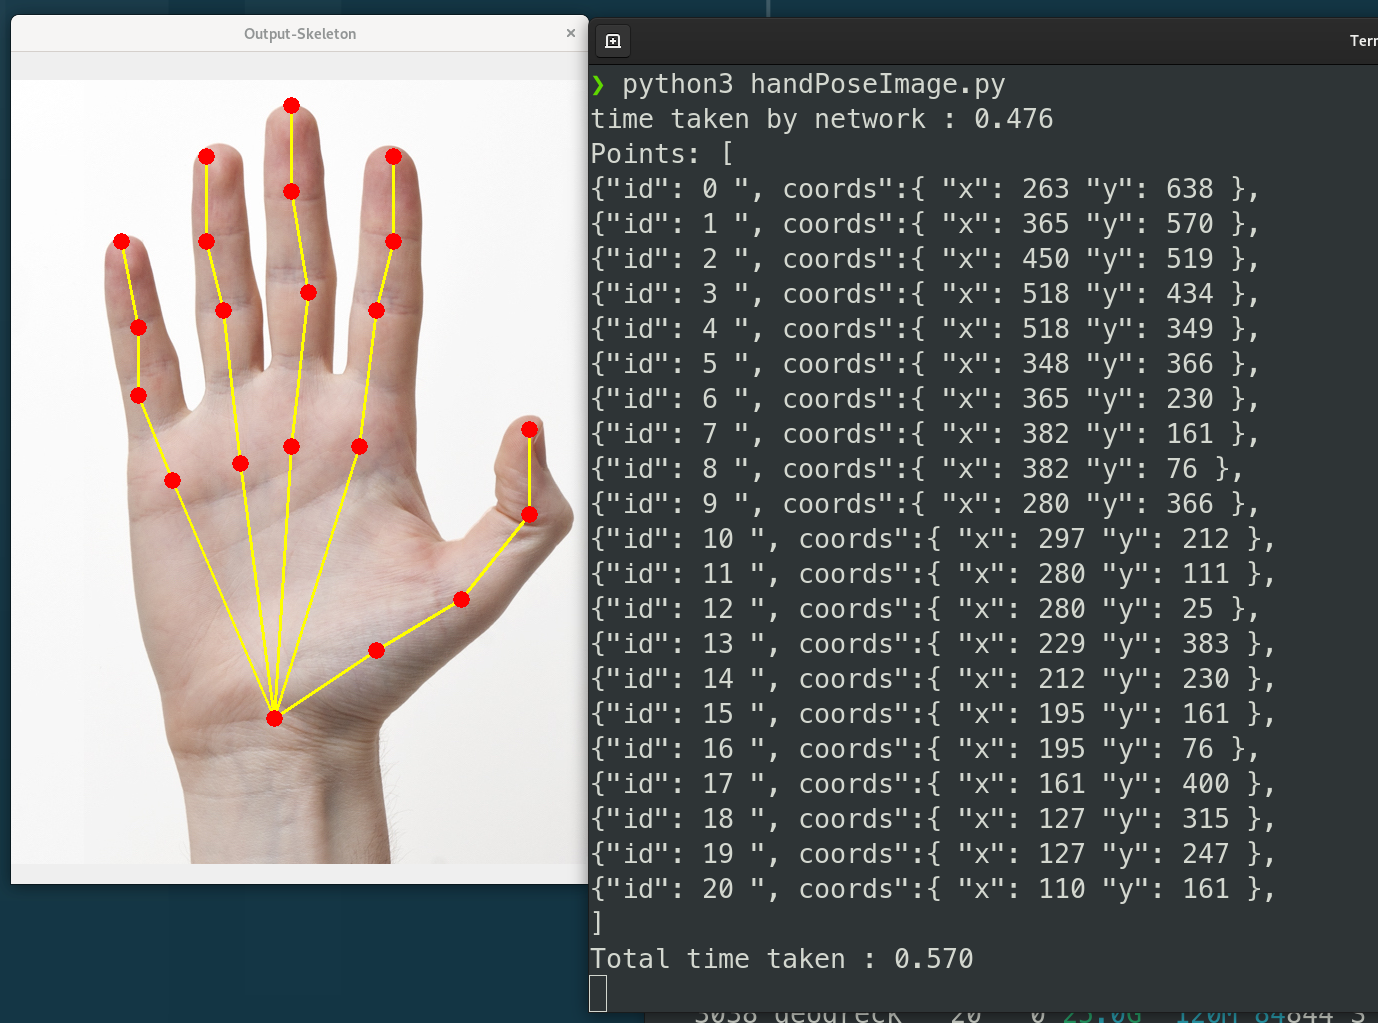
\includegraphics{pics/hw2_pythonHand_out.png}
\caption{Распознавание на Python}
\end{figure}

Исходный код на языке \textbf{\texttt{C++}}:

\begin{Shaded}
\begin{Highlighting}[numbers=left,,]
\PreprocessorTok{\#include }\ImportTok{\textless{}opencv2/dnn.hpp\textgreater{}}
\PreprocessorTok{\#include }\ImportTok{\textless{}opencv2/imgproc.hpp\textgreater{}}
\PreprocessorTok{\#include }\ImportTok{\textless{}opencv2/highgui.hpp\textgreater{}}
\PreprocessorTok{\#include }\ImportTok{\textless{}iostream\textgreater{}}

\KeywordTok{using} \KeywordTok{namespace}\NormalTok{ std;}
\KeywordTok{using} \KeywordTok{namespace}\NormalTok{ cv;}
\KeywordTok{using} \KeywordTok{namespace}\NormalTok{ cv::dnn;}


\AttributeTok{const} \DataTypeTok{int}\NormalTok{ POSE\_PAIRS[}\DecValTok{20}\NormalTok{][}\DecValTok{2}\NormalTok{] =}
\NormalTok{\{}
\NormalTok{    \{}\DecValTok{0}\NormalTok{,}\DecValTok{1}\NormalTok{\}, \{}\DecValTok{1}\NormalTok{,}\DecValTok{2}\NormalTok{\}, \{}\DecValTok{2}\NormalTok{,}\DecValTok{3}\NormalTok{\}, \{}\DecValTok{3}\NormalTok{,}\DecValTok{4}\NormalTok{\},         }\CommentTok{// thumb}
\NormalTok{    \{}\DecValTok{0}\NormalTok{,}\DecValTok{5}\NormalTok{\}, \{}\DecValTok{5}\NormalTok{,}\DecValTok{6}\NormalTok{\}, \{}\DecValTok{6}\NormalTok{,}\DecValTok{7}\NormalTok{\}, \{}\DecValTok{7}\NormalTok{,}\DecValTok{8}\NormalTok{\},         }\CommentTok{// index}
\NormalTok{    \{}\DecValTok{0}\NormalTok{,}\DecValTok{9}\NormalTok{\}, \{}\DecValTok{9}\NormalTok{,}\DecValTok{10}\NormalTok{\}, \{}\DecValTok{10}\NormalTok{,}\DecValTok{11}\NormalTok{\}, \{}\DecValTok{11}\NormalTok{,}\DecValTok{12}\NormalTok{\},    }\CommentTok{// middle}
\NormalTok{    \{}\DecValTok{0}\NormalTok{,}\DecValTok{13}\NormalTok{\}, \{}\DecValTok{13}\NormalTok{,}\DecValTok{14}\NormalTok{\}, \{}\DecValTok{14}\NormalTok{,}\DecValTok{15}\NormalTok{\}, \{}\DecValTok{15}\NormalTok{,}\DecValTok{16}\NormalTok{\},  }\CommentTok{// ring}
\NormalTok{    \{}\DecValTok{0}\NormalTok{,}\DecValTok{17}\NormalTok{\}, \{}\DecValTok{17}\NormalTok{,}\DecValTok{18}\NormalTok{\}, \{}\DecValTok{18}\NormalTok{,}\DecValTok{19}\NormalTok{\}, \{}\DecValTok{19}\NormalTok{,}\DecValTok{20}\NormalTok{\}   }\CommentTok{// small}
\NormalTok{\};}

\NormalTok{string protoFile = }\StringTok{"hand/pose\_deploy.prototxt"}\NormalTok{;}
\NormalTok{string weightsFile = }\StringTok{"hand/pose\_iter\_102000.caffemodel"}\NormalTok{;}

\DataTypeTok{int}\NormalTok{ nPoints = }\DecValTok{22}\NormalTok{;}

\DataTypeTok{int}\NormalTok{ main(}\DataTypeTok{int}\NormalTok{ argc, }\DataTypeTok{char}\NormalTok{ **argv)}
\NormalTok{\{}

\NormalTok{    cout \textless{}\textless{} }\StringTok{"USAGE : ./handPoseImage \textless{}imageFile\textgreater{} "}\NormalTok{ \textless{}\textless{} endl;}

\NormalTok{    string imageFile = }\StringTok{"right{-}frontal.jpg"}\NormalTok{;}
    \CommentTok{// Take arguments from commmand line}
    \ControlFlowTok{if}\NormalTok{ (argc == }\DecValTok{2}\NormalTok{)}
\NormalTok{    \{}
\NormalTok{      imageFile = argv[}\DecValTok{1}\NormalTok{];}
\NormalTok{    \}}

    \DataTypeTok{float}\NormalTok{ thresh = }\FloatTok{0.01}\NormalTok{;}

\NormalTok{    Mat frame = imread(imageFile);}
\NormalTok{    Mat frameCopy = frame.clone();}
    \DataTypeTok{int}\NormalTok{ frameWidth = frame.cols;}
    \DataTypeTok{int}\NormalTok{ frameHeight = frame.rows;}

    \DataTypeTok{float}\NormalTok{ aspect\_ratio = frameWidth/(}\DataTypeTok{float}\NormalTok{)frameHeight;}
    \DataTypeTok{int}\NormalTok{ inHeight = }\DecValTok{368}\NormalTok{;}
    \DataTypeTok{int}\NormalTok{ inWidth = (}\DataTypeTok{int}\NormalTok{(aspect\_ratio*inHeight) * }\DecValTok{8}\NormalTok{) / }\DecValTok{8}\NormalTok{;}

\NormalTok{    cout \textless{}\textless{} }\StringTok{"inWidth = "}\NormalTok{ \textless{}\textless{} inWidth \textless{}\textless{} }\StringTok{" ; inHeight = "}\NormalTok{ \textless{}\textless{} inHeight \textless{}\textless{} endl;}

    \DataTypeTok{double}\NormalTok{ t = (}\DataTypeTok{double}\NormalTok{) cv::getTickCount();}
\NormalTok{    Net net = readNetFromCaffe(protoFile, weightsFile);}

\NormalTok{    Mat inpBlob = blobFromImage(frame, }\FloatTok{1.0}\NormalTok{ / }\DecValTok{255}\NormalTok{, Size(inWidth, inHeight), Scalar(}\DecValTok{0}\NormalTok{, }\DecValTok{0}\NormalTok{, }\DecValTok{0}\NormalTok{), }\KeywordTok{false}\NormalTok{, }\KeywordTok{false}\NormalTok{);}

\NormalTok{    net.setInput(inpBlob);}

\NormalTok{    Mat output = net.forward();}

    \DataTypeTok{int}\NormalTok{ H = output.size[}\DecValTok{2}\NormalTok{];}
    \DataTypeTok{int}\NormalTok{ W = output.size[}\DecValTok{3}\NormalTok{];}

    \CommentTok{// find the position of the body parts}
\NormalTok{    vector\textless{}Point\textgreater{} points(nPoints);}
    \ControlFlowTok{for}\NormalTok{ (}\DataTypeTok{int}\NormalTok{ n=}\DecValTok{0}\NormalTok{; n \textless{} nPoints; n++)}
\NormalTok{    \{}
        \CommentTok{// Probability map of corresponding body\textquotesingle{}s part.}
\NormalTok{        Mat probMap(H, W, CV\_32F, output.ptr(}\DecValTok{0}\NormalTok{,n));}
\NormalTok{        resize(probMap, probMap, Size(frameWidth, frameHeight));}

\NormalTok{        Point maxLoc;}
        \DataTypeTok{double}\NormalTok{ prob;}
\NormalTok{        minMaxLoc(probMap, }\DecValTok{0}\NormalTok{, \&prob, }\DecValTok{0}\NormalTok{, \&maxLoc);}
        \ControlFlowTok{if}\NormalTok{ (prob \textgreater{} thresh)}
\NormalTok{        \{}
\NormalTok{            circle(frameCopy, cv::Point((}\DataTypeTok{int}\NormalTok{)maxLoc.x, (}\DataTypeTok{int}\NormalTok{)maxLoc.y), }\DecValTok{8}\NormalTok{, Scalar(}\DecValTok{0}\NormalTok{,}\DecValTok{255}\NormalTok{,}\DecValTok{255}\NormalTok{), {-}}\DecValTok{1}\NormalTok{);}
\NormalTok{            cv::putText(frameCopy, cv::format(}\StringTok{"}\SpecialCharTok{\%d}\StringTok{"}\NormalTok{, n), cv::Point((}\DataTypeTok{int}\NormalTok{)maxLoc.x, (}\DataTypeTok{int}\NormalTok{)maxLoc.y), cv::FONT\_HERSHEY\_COMPLEX, }\DecValTok{1}\NormalTok{, cv::Scalar(}\DecValTok{0}\NormalTok{, }\DecValTok{0}\NormalTok{, }\DecValTok{255}\NormalTok{), }\DecValTok{2}\NormalTok{);}

\NormalTok{        \}}
\NormalTok{        points[n] = maxLoc;}
\NormalTok{    \}}

    \DataTypeTok{int}\NormalTok{ nPairs = }\KeywordTok{sizeof}\NormalTok{(POSE\_PAIRS)/}\KeywordTok{sizeof}\NormalTok{(POSE\_PAIRS[}\DecValTok{0}\NormalTok{]);}

    \ControlFlowTok{if}\NormalTok{ (nPairs \textgreater{} }\DecValTok{0}\NormalTok{)\{}
\NormalTok{        cout\textless{}\textless{}}\StringTok{"Points: ["}\NormalTok{;}
\NormalTok{    \}}
    \ControlFlowTok{for}\NormalTok{ (}\DataTypeTok{int}\NormalTok{ n = }\DecValTok{0}\NormalTok{; n \textless{} nPairs; n++)}
\NormalTok{    \{}
        \CommentTok{// lookup 2 connected body/hand parts}
\NormalTok{        Point2f partA = points[POSE\_PAIRS[n][}\DecValTok{0}\NormalTok{]];}
\NormalTok{        Point2f partB = points[POSE\_PAIRS[n][}\DecValTok{1}\NormalTok{]];}

        \ControlFlowTok{if}\NormalTok{ (partA.x\textless{}=}\DecValTok{0}\NormalTok{ || partA.y\textless{}=}\DecValTok{0}\NormalTok{ || partB.x\textless{}=}\DecValTok{0}\NormalTok{ || partB.y\textless{}=}\DecValTok{0}\NormalTok{)}
            \ControlFlowTok{continue}\NormalTok{;}

\NormalTok{        cout\textless{}\textless{}}\StringTok{"\{}\SpecialCharTok{\textbackslash{}"}\StringTok{id}\SpecialCharTok{\textbackslash{}"}\StringTok{:"}\NormalTok{\textless{}\textless{} n \textless{}\textless{} }\StringTok{"}\SpecialCharTok{\textbackslash{}"}\StringTok{, coords}\SpecialCharTok{\textbackslash{}"}\StringTok{:\{"}\NormalTok{\textless{}\textless{} }\StringTok{"}\SpecialCharTok{\textbackslash{}"}\StringTok{x}\SpecialCharTok{\textbackslash{}"}\StringTok{:"}\NormalTok{\textless{}\textless{} points[n].x\textless{}\textless{} }\StringTok{"}\SpecialCharTok{\textbackslash{}"}\StringTok{y}\SpecialCharTok{\textbackslash{}"}\StringTok{:"}\NormalTok{\textless{}\textless{} points[n].y\textless{}\textless{} }\StringTok{"\}, "}\NormalTok{;}

\NormalTok{        line(frame, partA, partB, Scalar(}\DecValTok{0}\NormalTok{,}\DecValTok{255}\NormalTok{,}\DecValTok{255}\NormalTok{), }\DecValTok{8}\NormalTok{);}
\NormalTok{        circle(frame, partA, }\DecValTok{8}\NormalTok{, Scalar(}\DecValTok{0}\NormalTok{,}\DecValTok{0}\NormalTok{,}\DecValTok{255}\NormalTok{), {-}}\DecValTok{1}\NormalTok{);}
\NormalTok{        circle(frame, partB, }\DecValTok{8}\NormalTok{, Scalar(}\DecValTok{0}\NormalTok{,}\DecValTok{0}\NormalTok{,}\DecValTok{255}\NormalTok{), {-}}\DecValTok{1}\NormalTok{);}
\NormalTok{    \}}
    \ControlFlowTok{if}\NormalTok{ (nPairs \textgreater{} }\DecValTok{0}\NormalTok{)\{}
\NormalTok{        cout\textless{}\textless{}}\StringTok{"]}\SpecialCharTok{\textbackslash{}n}\StringTok{"}\NormalTok{;}
\NormalTok{    \}}

\NormalTok{    t = ((}\DataTypeTok{double}\NormalTok{)cv::getTickCount() {-} t)/cv::getTickFrequency();}
\NormalTok{    cout \textless{}\textless{} }\StringTok{"Time Taken = "}\NormalTok{ \textless{}\textless{} t \textless{}\textless{} endl;}
\NormalTok{    imshow(}\StringTok{"Output{-}Keypoints"}\NormalTok{, frameCopy);}
\NormalTok{    imshow(}\StringTok{"Output{-}Skeleton"}\NormalTok{, frame);}
\NormalTok{    imwrite(}\StringTok{"Output{-}Skeleton.jpg"}\NormalTok{, frame);}

\NormalTok{    waitKey();}

    \ControlFlowTok{return} \DecValTok{0}\NormalTok{;}
\NormalTok{\}}
\end{Highlighting}
\end{Shaded}

\begin{figure}
\centering
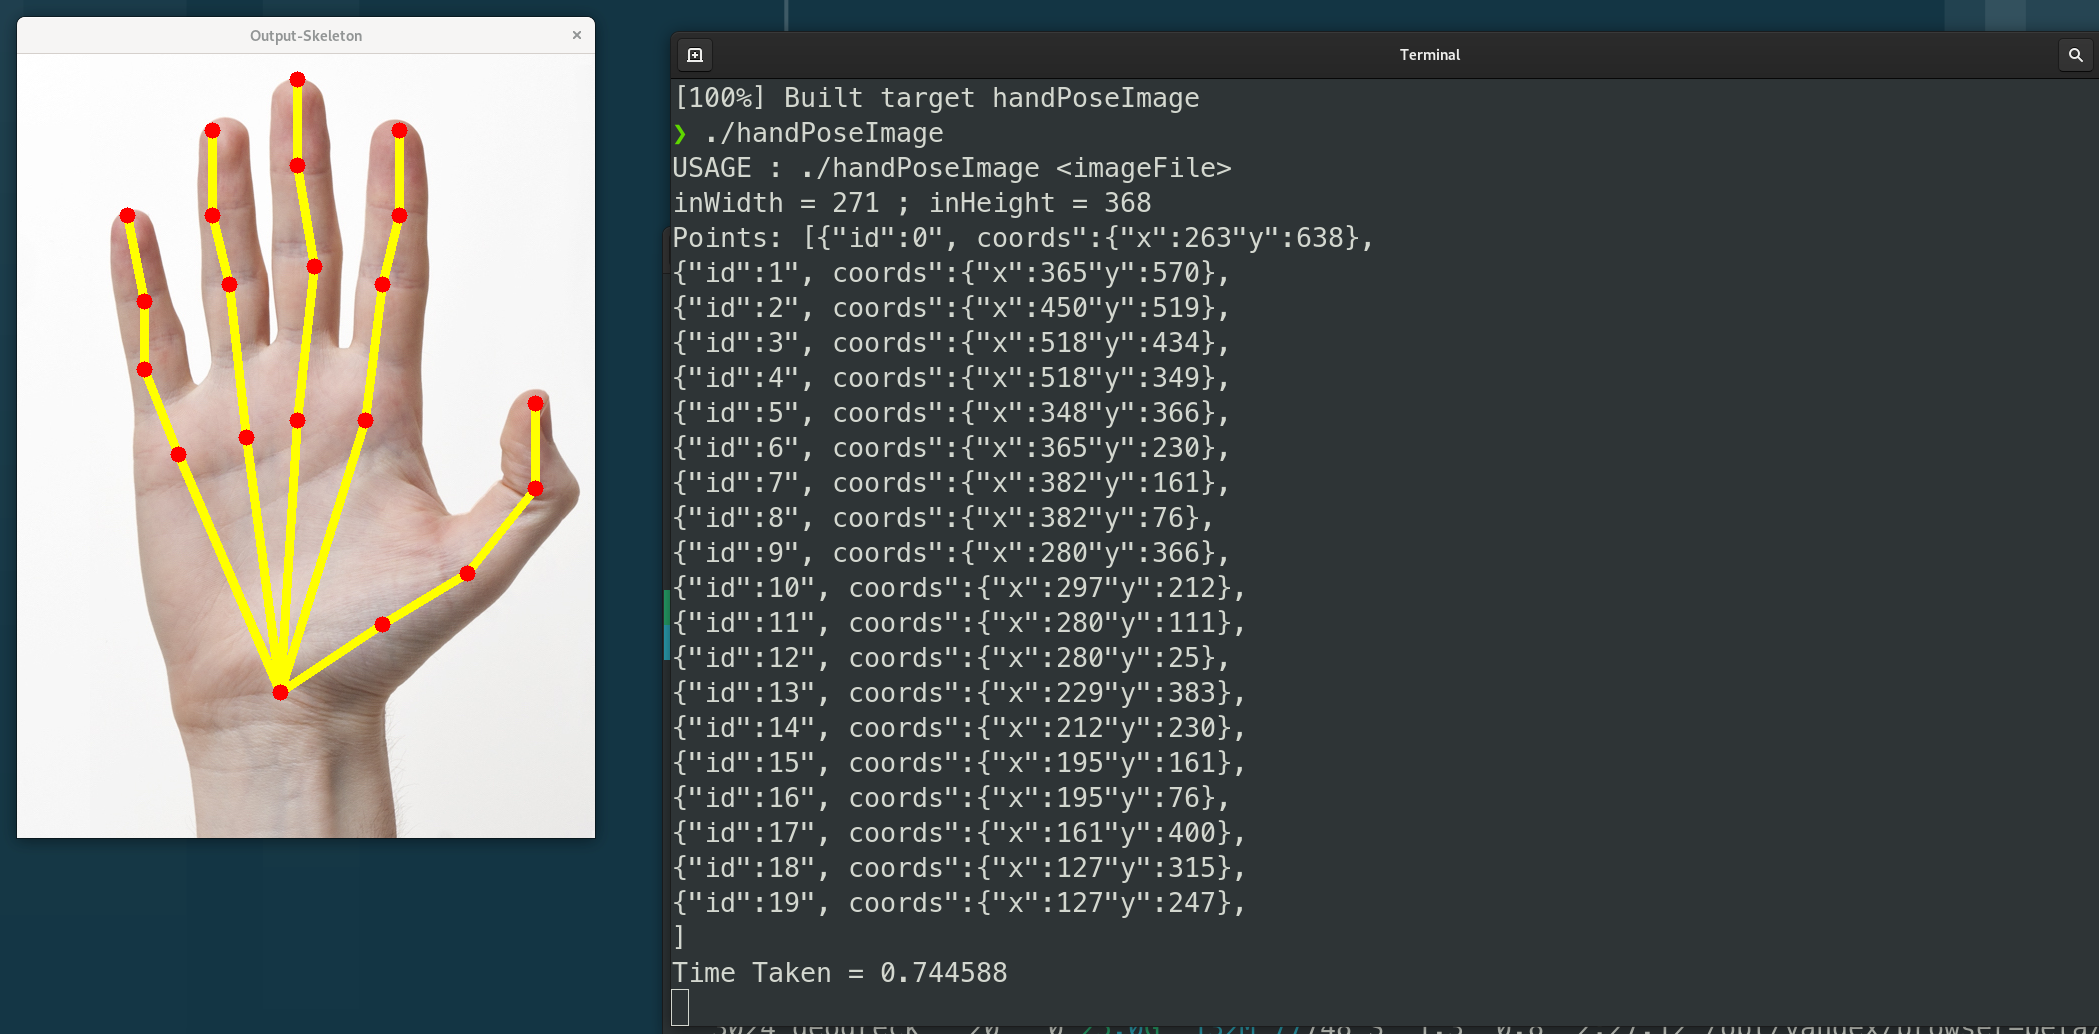
\includegraphics{pics/hw2_cppHand_out.png}
\caption{Распознавание на C++}
\end{figure}

\hypertarget{ux440ux430ux441ux43fux43eux437ux43dux43eux432ux430ux43dux438ux435-ux442ux43eux447ux435ux43a-ux442ux435ux43bux430}{%
\subsection{Распознование точек
тела}\label{ux440ux430ux441ux43fux43eux437ux43dux43eux432ux430ux43dux438ux435-ux442ux43eux447ux435ux43a-ux442ux435ux43bux430}}

Исходный код на \textbf{\texttt{Python}}:

\begin{Shaded}
\begin{Highlighting}[numbers=left,,]
\ImportTok{import}\NormalTok{ cv2}
\ImportTok{import}\NormalTok{ time}
\ImportTok{import}\NormalTok{ numpy }\ImportTok{as}\NormalTok{ np}
\ImportTok{import}\NormalTok{ argparse}

\NormalTok{parser }\OperatorTok{=}\NormalTok{ argparse.ArgumentParser(description}\OperatorTok{=}\StringTok{\textquotesingle{}Run keypoint detection\textquotesingle{}}\NormalTok{)}
\NormalTok{parser.add\_argument(}\StringTok{"{-}{-}device"}\NormalTok{, default}\OperatorTok{=}\StringTok{"cpu"}\NormalTok{, }\BuiltInTok{help}\OperatorTok{=}\StringTok{"Device to inference on"}\NormalTok{)}
\NormalTok{parser.add\_argument(}\StringTok{"{-}{-}image\_file"}\NormalTok{, default}\OperatorTok{=}\StringTok{"single.jpeg"}\NormalTok{, }\BuiltInTok{help}\OperatorTok{=}\StringTok{"Input image"}\NormalTok{)}

\NormalTok{args }\OperatorTok{=}\NormalTok{ parser.parse\_args()}


\NormalTok{MODE }\OperatorTok{=} \StringTok{"COCO"}

\ControlFlowTok{if}\NormalTok{ MODE }\KeywordTok{is} \StringTok{"COCO"}\NormalTok{:}
\NormalTok{    protoFile }\OperatorTok{=} \StringTok{"pose/coco/pose\_deploy\_linevec.prototxt"}
\NormalTok{    weightsFile }\OperatorTok{=} \StringTok{"pose/coco/pose\_iter\_440000.caffemodel"}
\NormalTok{    nPoints }\OperatorTok{=} \DecValTok{18}
\NormalTok{    POSE\_PAIRS }\OperatorTok{=}\NormalTok{ [ [}\DecValTok{1}\NormalTok{,}\DecValTok{0}\NormalTok{],[}\DecValTok{1}\NormalTok{,}\DecValTok{2}\NormalTok{],[}\DecValTok{1}\NormalTok{,}\DecValTok{5}\NormalTok{],[}\DecValTok{2}\NormalTok{,}\DecValTok{3}\NormalTok{],[}\DecValTok{3}\NormalTok{,}\DecValTok{4}\NormalTok{],[}\DecValTok{5}\NormalTok{,}\DecValTok{6}\NormalTok{],[}\DecValTok{6}\NormalTok{,}\DecValTok{7}\NormalTok{],[}\DecValTok{1}\NormalTok{,}\DecValTok{8}\NormalTok{],[}\DecValTok{8}\NormalTok{,}\DecValTok{9}\NormalTok{],[}\DecValTok{9}\NormalTok{,}\DecValTok{10}\NormalTok{],[}\DecValTok{1}\NormalTok{,}\DecValTok{11}\NormalTok{],[}\DecValTok{11}\NormalTok{,}\DecValTok{12}\NormalTok{],[}\DecValTok{12}\NormalTok{,}\DecValTok{13}\NormalTok{],[}\DecValTok{0}\NormalTok{,}\DecValTok{14}\NormalTok{],[}\DecValTok{0}\NormalTok{,}\DecValTok{15}\NormalTok{],[}\DecValTok{14}\NormalTok{,}\DecValTok{16}\NormalTok{],[}\DecValTok{15}\NormalTok{,}\DecValTok{17}\NormalTok{]]}

\ControlFlowTok{elif}\NormalTok{ MODE }\KeywordTok{is} \StringTok{"MPI"}\NormalTok{ :}
\NormalTok{    protoFile }\OperatorTok{=} \StringTok{"pose/mpi/pose\_deploy\_linevec\_faster\_4\_stages.prototxt"}
\NormalTok{    weightsFile }\OperatorTok{=} \StringTok{"pose/mpi/pose\_iter\_160000.caffemodel"}
\NormalTok{    nPoints }\OperatorTok{=} \DecValTok{15}
\NormalTok{    POSE\_PAIRS }\OperatorTok{=}\NormalTok{ [[}\DecValTok{0}\NormalTok{,}\DecValTok{1}\NormalTok{], [}\DecValTok{1}\NormalTok{,}\DecValTok{2}\NormalTok{], [}\DecValTok{2}\NormalTok{,}\DecValTok{3}\NormalTok{], [}\DecValTok{3}\NormalTok{,}\DecValTok{4}\NormalTok{], [}\DecValTok{1}\NormalTok{,}\DecValTok{5}\NormalTok{], [}\DecValTok{5}\NormalTok{,}\DecValTok{6}\NormalTok{], [}\DecValTok{6}\NormalTok{,}\DecValTok{7}\NormalTok{], [}\DecValTok{1}\NormalTok{,}\DecValTok{14}\NormalTok{], [}\DecValTok{14}\NormalTok{,}\DecValTok{8}\NormalTok{], [}\DecValTok{8}\NormalTok{,}\DecValTok{9}\NormalTok{], [}\DecValTok{9}\NormalTok{,}\DecValTok{10}\NormalTok{], [}\DecValTok{14}\NormalTok{,}\DecValTok{11}\NormalTok{], [}\DecValTok{11}\NormalTok{,}\DecValTok{12}\NormalTok{], [}\DecValTok{12}\NormalTok{,}\DecValTok{13}\NormalTok{] ]}


\NormalTok{frame }\OperatorTok{=}\NormalTok{ cv2.imread(args.image\_file)}
\NormalTok{frameCopy }\OperatorTok{=}\NormalTok{ np.copy(frame)}
\NormalTok{frameWidth }\OperatorTok{=}\NormalTok{ frame.shape[}\DecValTok{1}\NormalTok{]}
\NormalTok{frameHeight }\OperatorTok{=}\NormalTok{ frame.shape[}\DecValTok{0}\NormalTok{]}
\NormalTok{threshold }\OperatorTok{=} \FloatTok{0.1}

\NormalTok{net }\OperatorTok{=}\NormalTok{ cv2.dnn.readNetFromCaffe(protoFile, weightsFile)}

\ControlFlowTok{if}\NormalTok{ args.device }\OperatorTok{==} \StringTok{"cpu"}\NormalTok{:}
\NormalTok{    net.setPreferableBackend(cv2.dnn.DNN\_TARGET\_CPU)}
    \BuiltInTok{print}\NormalTok{(}\StringTok{"Using CPU device"}\NormalTok{)}
\ControlFlowTok{elif}\NormalTok{ args.device }\OperatorTok{==} \StringTok{"gpu"}\NormalTok{:}
\NormalTok{    net.setPreferableBackend(cv2.dnn.DNN\_BACKEND\_CUDA)}
\NormalTok{    net.setPreferableTarget(cv2.dnn.DNN\_TARGET\_CUDA)}
    \BuiltInTok{print}\NormalTok{(}\StringTok{"Using GPU device"}\NormalTok{)}

\NormalTok{t }\OperatorTok{=}\NormalTok{ time.time()}
\CommentTok{\# input image dimensions for the network}
\NormalTok{inWidth }\OperatorTok{=} \DecValTok{368}
\NormalTok{inHeight }\OperatorTok{=} \DecValTok{368}
\NormalTok{inpBlob }\OperatorTok{=}\NormalTok{ cv2.dnn.blobFromImage(frame, }\FloatTok{1.0} \OperatorTok{/} \DecValTok{255}\NormalTok{, (inWidth, inHeight),}
\NormalTok{                          (}\DecValTok{0}\NormalTok{, }\DecValTok{0}\NormalTok{, }\DecValTok{0}\NormalTok{), swapRB}\OperatorTok{=}\VariableTok{False}\NormalTok{, crop}\OperatorTok{=}\VariableTok{False}\NormalTok{)}

\NormalTok{net.setInput(inpBlob)}

\NormalTok{output }\OperatorTok{=}\NormalTok{ net.forward()}
\BuiltInTok{print}\NormalTok{(}\StringTok{"time taken by network : }\SpecialCharTok{\{:.3f\}}\StringTok{"}\NormalTok{.}\BuiltInTok{format}\NormalTok{(time.time() }\OperatorTok{{-}}\NormalTok{ t))}

\NormalTok{H }\OperatorTok{=}\NormalTok{ output.shape[}\DecValTok{2}\NormalTok{]}
\NormalTok{W }\OperatorTok{=}\NormalTok{ output.shape[}\DecValTok{3}\NormalTok{]}

\CommentTok{\# Empty list to store the detected keypoints}
\NormalTok{points }\OperatorTok{=}\NormalTok{ []}
\NormalTok{count }\OperatorTok{=} \DecValTok{0}

\ControlFlowTok{for}\NormalTok{ i }\KeywordTok{in} \BuiltInTok{range}\NormalTok{(nPoints):}
    \CommentTok{\# confidence map of corresponding body\textquotesingle{}s part.}
\NormalTok{    probMap }\OperatorTok{=}\NormalTok{ output[}\DecValTok{0}\NormalTok{, i, :, :]}

    \CommentTok{\# Find global maxima of the probMap.}
\NormalTok{    minVal, prob, minLoc, point }\OperatorTok{=}\NormalTok{ cv2.minMaxLoc(probMap)}
    
    \CommentTok{\# Scale the point to fit on the original image}
\NormalTok{    x }\OperatorTok{=}\NormalTok{ (frameWidth }\OperatorTok{*}\NormalTok{ point[}\DecValTok{0}\NormalTok{]) }\OperatorTok{/}\NormalTok{ W}
\NormalTok{    y }\OperatorTok{=}\NormalTok{ (frameHeight }\OperatorTok{*}\NormalTok{ point[}\DecValTok{1}\NormalTok{]) }\OperatorTok{/}\NormalTok{ H}

    \ControlFlowTok{if}\NormalTok{ prob }\OperatorTok{\textgreater{}}\NormalTok{ threshold : }
\NormalTok{        cv2.circle(frameCopy, (}\BuiltInTok{int}\NormalTok{(x), }\BuiltInTok{int}\NormalTok{(y)), }\DecValTok{8}\NormalTok{, (}\DecValTok{0}\NormalTok{, }\DecValTok{255}\NormalTok{, }\DecValTok{255}\NormalTok{), thickness}\OperatorTok{={-}}\DecValTok{1}\NormalTok{, lineType}\OperatorTok{=}\NormalTok{cv2.FILLED)}
\NormalTok{        cv2.putText(frameCopy, }\StringTok{"}\SpecialCharTok{\{\}}\StringTok{"}\NormalTok{.}\BuiltInTok{format}\NormalTok{(i), (}\BuiltInTok{int}\NormalTok{(x), }\BuiltInTok{int}\NormalTok{(y)), cv2.FONT\_HERSHEY\_SIMPLEX, }\DecValTok{1}\NormalTok{, (}\DecValTok{0}\NormalTok{, }\DecValTok{0}\NormalTok{, }\DecValTok{255}\NormalTok{), }\DecValTok{2}\NormalTok{, lineType}\OperatorTok{=}\NormalTok{cv2.LINE\_AA)}

        \CommentTok{\# Add the point to the list if the probability is greater than the threshold}
\NormalTok{        points.append((}\BuiltInTok{int}\NormalTok{(x), }\BuiltInTok{int}\NormalTok{(y)))}
\NormalTok{        count}\OperatorTok{+=}\DecValTok{1}
    \ControlFlowTok{else}\NormalTok{ :}
\NormalTok{        points.append(}\VariableTok{None}\NormalTok{)}

\CommentTok{\# JSON output}
\ControlFlowTok{if}\NormalTok{ count }\OperatorTok{\textgreater{}} \DecValTok{1}\NormalTok{:}
    \BuiltInTok{print}\NormalTok{ (}\StringTok{"Points: ["}\NormalTok{)}
\NormalTok{    i }\OperatorTok{=} \DecValTok{0}
\NormalTok{    k }\OperatorTok{=} \DecValTok{0}
    \ControlFlowTok{while}\NormalTok{ k }\OperatorTok{\textless{}}\NormalTok{ count:}
        \ControlFlowTok{if}\NormalTok{ points[i] }\OperatorTok{!=} \VariableTok{None}\NormalTok{:}
            \BuiltInTok{print}\NormalTok{ (}\StringTok{"\{}\CharTok{\textbackslash{}"}\StringTok{id}\CharTok{\textbackslash{}"}\StringTok{:"}\NormalTok{, k, }\StringTok{"}\CharTok{\textbackslash{}"}\StringTok{, coords}\CharTok{\textbackslash{}"}\StringTok{:\{"}\NormalTok{, }\StringTok{"}\CharTok{\textbackslash{}"}\StringTok{x}\CharTok{\textbackslash{}"}\StringTok{:"}\NormalTok{, points[i][}\DecValTok{0}\NormalTok{], }\StringTok{"}\CharTok{\textbackslash{}"}\StringTok{y}\CharTok{\textbackslash{}"}\StringTok{:"}\NormalTok{, points[i][}\DecValTok{1}\NormalTok{], }\StringTok{"\}, "}\NormalTok{)}
\NormalTok{            k}\OperatorTok{+=}\DecValTok{1}
\NormalTok{        i}\OperatorTok{+=}\DecValTok{1}    
    \CommentTok{\#print ("\{\textbackslash{}"id\textbackslash{}":", count {-} 1, "\textbackslash{}", coords\textbackslash{}":\{", "\textbackslash{}"x\textbackslash{}":", points[count {-} 1][0], "\textbackslash{}"y\textbackslash{}":", points[count {-} 1][1], "\} ")}
    \BuiltInTok{print}\NormalTok{ (}\StringTok{"]"}\NormalTok{)}

\CommentTok{\# Draw Skeleton}
\ControlFlowTok{for}\NormalTok{ pair }\KeywordTok{in}\NormalTok{ POSE\_PAIRS:}
\NormalTok{    partA }\OperatorTok{=}\NormalTok{ pair[}\DecValTok{0}\NormalTok{]}
\NormalTok{    partB }\OperatorTok{=}\NormalTok{ pair[}\DecValTok{1}\NormalTok{]}

    \ControlFlowTok{if}\NormalTok{ points[partA] }\KeywordTok{and}\NormalTok{ points[partB]:}
\NormalTok{        cv2.line(frame, points[partA], points[partB], (}\DecValTok{0}\NormalTok{, }\DecValTok{255}\NormalTok{, }\DecValTok{255}\NormalTok{), }\DecValTok{2}\NormalTok{)}
\NormalTok{        cv2.circle(frame, points[partA], }\DecValTok{8}\NormalTok{, (}\DecValTok{0}\NormalTok{, }\DecValTok{0}\NormalTok{, }\DecValTok{255}\NormalTok{), thickness}\OperatorTok{={-}}\DecValTok{1}\NormalTok{, lineType}\OperatorTok{=}\NormalTok{cv2.FILLED)}


\NormalTok{cv2.imshow(}\StringTok{\textquotesingle{}Output{-}Keypoints\textquotesingle{}}\NormalTok{, frameCopy)}
\NormalTok{cv2.imshow(}\StringTok{\textquotesingle{}Output{-}Skeleton\textquotesingle{}}\NormalTok{, frame)}


\NormalTok{cv2.imwrite(}\StringTok{\textquotesingle{}Output{-}Keypoints.jpg\textquotesingle{}}\NormalTok{, frameCopy)}
\NormalTok{cv2.imwrite(}\StringTok{\textquotesingle{}Output{-}Skeleton.jpg\textquotesingle{}}\NormalTok{, frame)}

\BuiltInTok{print}\NormalTok{(}\StringTok{"Total time taken : }\SpecialCharTok{\{:.3f\}}\StringTok{"}\NormalTok{.}\BuiltInTok{format}\NormalTok{(time.time() }\OperatorTok{{-}}\NormalTok{ t))}

\NormalTok{cv2.waitKey(}\DecValTok{0}\NormalTok{)}
\end{Highlighting}
\end{Shaded}

\begin{figure}
\centering
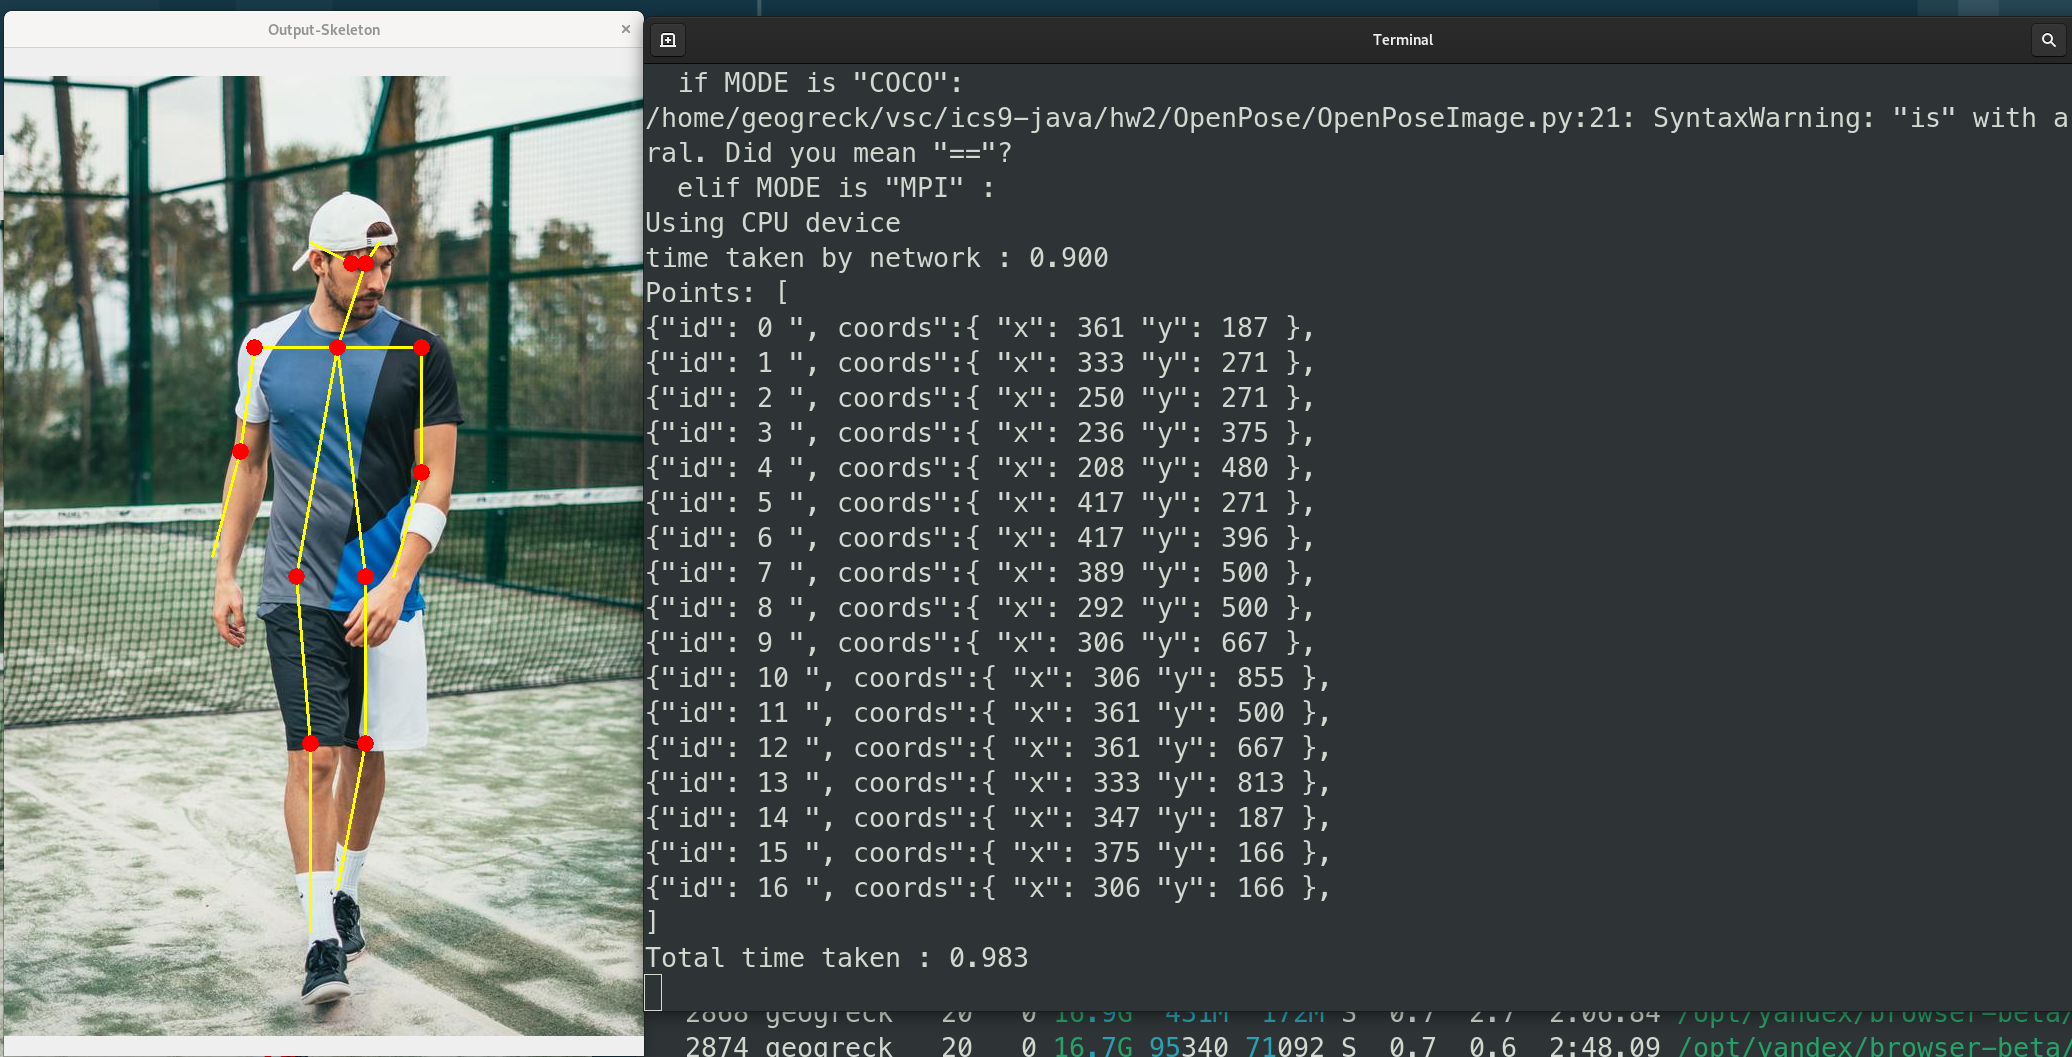
\includegraphics{pics/hw2_pythonBody_out.png}
\caption{Распознование на Python}
\end{figure}

Исходный код на \textbf{\texttt{С++}}:

\begin{Shaded}
\begin{Highlighting}[numbers=left,,]
\PreprocessorTok{\#include }\ImportTok{\textless{}opencv2/dnn.hpp\textgreater{}}
\PreprocessorTok{\#include }\ImportTok{\textless{}opencv2/imgproc.hpp\textgreater{}}
\PreprocessorTok{\#include }\ImportTok{\textless{}opencv2/highgui.hpp\textgreater{}}
\PreprocessorTok{\#include }\ImportTok{\textless{}iostream\textgreater{}}

\KeywordTok{using} \KeywordTok{namespace}\NormalTok{ std;}
\KeywordTok{using} \KeywordTok{namespace}\NormalTok{ cv;}
\KeywordTok{using} \KeywordTok{namespace}\NormalTok{ cv::dnn;}

\PreprocessorTok{\#define MPI}

\PreprocessorTok{\#ifdef MPI}
\AttributeTok{const} \DataTypeTok{int}\NormalTok{ POSE\_PAIRS[}\DecValTok{14}\NormalTok{][}\DecValTok{2}\NormalTok{] = }
\NormalTok{\{   }
\NormalTok{    \{}\DecValTok{0}\NormalTok{,}\DecValTok{1}\NormalTok{\}, \{}\DecValTok{1}\NormalTok{,}\DecValTok{2}\NormalTok{\}, \{}\DecValTok{2}\NormalTok{,}\DecValTok{3}\NormalTok{\},}
\NormalTok{    \{}\DecValTok{3}\NormalTok{,}\DecValTok{4}\NormalTok{\}, \{}\DecValTok{1}\NormalTok{,}\DecValTok{5}\NormalTok{\}, \{}\DecValTok{5}\NormalTok{,}\DecValTok{6}\NormalTok{\},}
\NormalTok{    \{}\DecValTok{6}\NormalTok{,}\DecValTok{7}\NormalTok{\}, \{}\DecValTok{1}\NormalTok{,}\DecValTok{14}\NormalTok{\}, \{}\DecValTok{14}\NormalTok{,}\DecValTok{8}\NormalTok{\}, \{}\DecValTok{8}\NormalTok{,}\DecValTok{9}\NormalTok{\},}
\NormalTok{    \{}\DecValTok{9}\NormalTok{,}\DecValTok{10}\NormalTok{\}, \{}\DecValTok{14}\NormalTok{,}\DecValTok{11}\NormalTok{\}, \{}\DecValTok{11}\NormalTok{,}\DecValTok{12}\NormalTok{\}, \{}\DecValTok{12}\NormalTok{,}\DecValTok{13}\NormalTok{\}}
\NormalTok{\};}

\NormalTok{string protoFile = }\StringTok{"pose/mpi/pose\_deploy\_linevec\_faster\_4\_stages.prototxt"}\NormalTok{;}
\NormalTok{string weightsFile = }\StringTok{"pose/mpi/pose\_iter\_160000.caffemodel"}\NormalTok{;}

\DataTypeTok{int}\NormalTok{ nPoints = }\DecValTok{15}\NormalTok{;}
\PreprocessorTok{\#endif}

\PreprocessorTok{\#ifdef COCO}
\AttributeTok{const} \DataTypeTok{int}\NormalTok{ POSE\_PAIRS[}\DecValTok{17}\NormalTok{][}\DecValTok{2}\NormalTok{] = }
\NormalTok{\{   }
\NormalTok{    \{}\DecValTok{1}\NormalTok{,}\DecValTok{2}\NormalTok{\}, \{}\DecValTok{1}\NormalTok{,}\DecValTok{5}\NormalTok{\}, \{}\DecValTok{2}\NormalTok{,}\DecValTok{3}\NormalTok{\},}
\NormalTok{    \{}\DecValTok{3}\NormalTok{,}\DecValTok{4}\NormalTok{\}, \{}\DecValTok{5}\NormalTok{,}\DecValTok{6}\NormalTok{\}, \{}\DecValTok{6}\NormalTok{,}\DecValTok{7}\NormalTok{\},}
\NormalTok{    \{}\DecValTok{1}\NormalTok{,}\DecValTok{8}\NormalTok{\}, \{}\DecValTok{8}\NormalTok{,}\DecValTok{9}\NormalTok{\}, \{}\DecValTok{9}\NormalTok{,}\DecValTok{10}\NormalTok{\},}
\NormalTok{    \{}\DecValTok{1}\NormalTok{,}\DecValTok{11}\NormalTok{\}, \{}\DecValTok{11}\NormalTok{,}\DecValTok{12}\NormalTok{\}, \{}\DecValTok{12}\NormalTok{,}\DecValTok{13}\NormalTok{\},}
\NormalTok{    \{}\DecValTok{1}\NormalTok{,}\DecValTok{0}\NormalTok{\}, \{}\DecValTok{0}\NormalTok{,}\DecValTok{14}\NormalTok{\},}
\NormalTok{    \{}\DecValTok{14}\NormalTok{,}\DecValTok{16}\NormalTok{\}, \{}\DecValTok{0}\NormalTok{,}\DecValTok{15}\NormalTok{\}, \{}\DecValTok{15}\NormalTok{,}\DecValTok{17}\NormalTok{\}}
\NormalTok{\};}

\NormalTok{string protoFile = }\StringTok{"pose/coco/pose\_deploy\_linevec.prototxt"}\NormalTok{;}
\NormalTok{string weightsFile = }\StringTok{"pose/coco/pose\_iter\_440000.caffemodel"}\NormalTok{;}

\DataTypeTok{int}\NormalTok{ nPoints = }\DecValTok{18}\NormalTok{;}
\PreprocessorTok{\#endif}

\DataTypeTok{int}\NormalTok{ main(}\DataTypeTok{int}\NormalTok{ argc, }\DataTypeTok{char}\NormalTok{ **argv)}
\NormalTok{\{}

\NormalTok{    cout \textless{}\textless{} }\StringTok{"USAGE : ./OpenPose \textless{}imageFile\textgreater{} "}\NormalTok{ \textless{}\textless{} endl;}
\NormalTok{    cout \textless{}\textless{} }\StringTok{"USAGE : ./OpenPose \textless{}imageFile\textgreater{} \textless{}device\textgreater{}"}\NormalTok{ \textless{}\textless{} endl;}
    
\NormalTok{    string device = }\StringTok{"cpu"}\NormalTok{;}

\NormalTok{    string imageFile = }\StringTok{"single.jpeg"}\NormalTok{;}
    \CommentTok{// Take arguments from commmand line}
    \ControlFlowTok{if}\NormalTok{ (argc == }\DecValTok{2}\NormalTok{)}
\NormalTok{    \{   }
      \ControlFlowTok{if}\NormalTok{((string)argv[}\DecValTok{1}\NormalTok{] == }\StringTok{"gpu"}\NormalTok{)}
\NormalTok{        device = }\StringTok{"gpu"}\NormalTok{;}
      \ControlFlowTok{else} 
\NormalTok{      imageFile = argv[}\DecValTok{1}\NormalTok{];}
\NormalTok{    \}}
    \ControlFlowTok{else} \ControlFlowTok{if}\NormalTok{ (argc == }\DecValTok{3}\NormalTok{)}
\NormalTok{    \{}
\NormalTok{        imageFile = argv[}\DecValTok{1}\NormalTok{];}
        \ControlFlowTok{if}\NormalTok{((string)argv[}\DecValTok{2}\NormalTok{] == }\StringTok{"gpu"}\NormalTok{)}
\NormalTok{            device = }\StringTok{"gpu"}\NormalTok{;}
\NormalTok{    \}}



    \DataTypeTok{int}\NormalTok{ inWidth = }\DecValTok{368}\NormalTok{;}
    \DataTypeTok{int}\NormalTok{ inHeight = }\DecValTok{368}\NormalTok{;}
    \DataTypeTok{float}\NormalTok{ thresh = }\FloatTok{0.1}\NormalTok{;    }

\NormalTok{    Mat frame = imread(imageFile);}
\NormalTok{    Mat frameCopy = frame.clone();}
    \DataTypeTok{int}\NormalTok{ frameWidth = frame.cols;}
    \DataTypeTok{int}\NormalTok{ frameHeight = frame.rows;}

    \DataTypeTok{double}\NormalTok{ t = (}\DataTypeTok{double}\NormalTok{) cv::getTickCount();}
\NormalTok{    Net net = readNetFromCaffe(protoFile, weightsFile);}

    \ControlFlowTok{if}\NormalTok{ (device == }\StringTok{"cpu"}\NormalTok{)}
\NormalTok{    \{}
\NormalTok{        cout \textless{}\textless{} }\StringTok{"Using CPU device"}\NormalTok{ \textless{}\textless{} endl;}
\NormalTok{        net.setPreferableBackend(DNN\_TARGET\_CPU);}
\NormalTok{    \}}
    \ControlFlowTok{else} \ControlFlowTok{if}\NormalTok{ (device == }\StringTok{"gpu"}\NormalTok{)}
\NormalTok{    \{}
\NormalTok{        cout \textless{}\textless{} }\StringTok{"Using GPU device"}\NormalTok{ \textless{}\textless{} endl;}
\NormalTok{        net.setPreferableBackend(DNN\_BACKEND\_CUDA);}
\NormalTok{        net.setPreferableTarget(DNN\_TARGET\_CUDA);}
\NormalTok{    \}}

\NormalTok{    Mat inpBlob = blobFromImage(frame, }\FloatTok{1.0}\NormalTok{ / }\DecValTok{255}\NormalTok{, Size(inWidth, inHeight), Scalar(}\DecValTok{0}\NormalTok{, }\DecValTok{0}\NormalTok{, }\DecValTok{0}\NormalTok{), }\KeywordTok{false}\NormalTok{, }\KeywordTok{false}\NormalTok{);}

\NormalTok{    net.setInput(inpBlob);}

\NormalTok{    Mat output = net.forward();}

    \DataTypeTok{int}\NormalTok{ H = output.size[}\DecValTok{2}\NormalTok{];}
    \DataTypeTok{int}\NormalTok{ W = output.size[}\DecValTok{3}\NormalTok{];}

    \CommentTok{// find the position of the body parts}
\NormalTok{    vector\textless{}Point\textgreater{} points(nPoints);}
    \ControlFlowTok{for}\NormalTok{ (}\DataTypeTok{int}\NormalTok{ n=}\DecValTok{0}\NormalTok{; n \textless{} nPoints; n++)}
\NormalTok{    \{}
        \CommentTok{// Probability map of corresponding body\textquotesingle{}s part.}
\NormalTok{        Mat probMap(H, W, CV\_32F, output.ptr(}\DecValTok{0}\NormalTok{,n));}

\NormalTok{        Point2f p({-}}\DecValTok{1}\NormalTok{,{-}}\DecValTok{1}\NormalTok{);}
\NormalTok{        Point maxLoc;}
        \DataTypeTok{double}\NormalTok{ prob;}
\NormalTok{        minMaxLoc(probMap, }\DecValTok{0}\NormalTok{, \&prob, }\DecValTok{0}\NormalTok{, \&maxLoc);}
        \ControlFlowTok{if}\NormalTok{ (prob \textgreater{} thresh)}
\NormalTok{        \{}
\NormalTok{            p = maxLoc;}
\NormalTok{            p.x *= (}\DataTypeTok{float}\NormalTok{)frameWidth / W ;}
\NormalTok{            p.y *= (}\DataTypeTok{float}\NormalTok{)frameHeight / H ;}

\NormalTok{            circle(frameCopy, cv::Point((}\DataTypeTok{int}\NormalTok{)p.x, (}\DataTypeTok{int}\NormalTok{)p.y), }\DecValTok{8}\NormalTok{, Scalar(}\DecValTok{0}\NormalTok{,}\DecValTok{255}\NormalTok{,}\DecValTok{255}\NormalTok{), {-}}\DecValTok{1}\NormalTok{);}
\NormalTok{            cv::putText(frameCopy, cv::format(}\StringTok{"}\SpecialCharTok{\%d}\StringTok{"}\NormalTok{, n), cv::Point((}\DataTypeTok{int}\NormalTok{)p.x, (}\DataTypeTok{int}\NormalTok{)p.y), cv::FONT\_HERSHEY\_COMPLEX, }\DecValTok{1}\NormalTok{, cv::Scalar(}\DecValTok{0}\NormalTok{, }\DecValTok{0}\NormalTok{, }\DecValTok{255}\NormalTok{), }\DecValTok{2}\NormalTok{);}

\NormalTok{        \}}
\NormalTok{        points[n] = p;}
\NormalTok{    \}}

    \DataTypeTok{int}\NormalTok{ nPairs = }\KeywordTok{sizeof}\NormalTok{(POSE\_PAIRS)/}\KeywordTok{sizeof}\NormalTok{(POSE\_PAIRS[}\DecValTok{0}\NormalTok{]);}

    \ControlFlowTok{if}\NormalTok{ (nPairs \textgreater{} }\DecValTok{0}\NormalTok{)\{}
\NormalTok{        cout\textless{}\textless{}}\StringTok{"Points: ["}\NormalTok{;}
\NormalTok{    \}}
    \ControlFlowTok{for}\NormalTok{ (}\DataTypeTok{int}\NormalTok{ n = }\DecValTok{0}\NormalTok{; n \textless{} nPairs; n++)}
\NormalTok{    \{}
        \CommentTok{// lookup 2 connected body/hand parts}
\NormalTok{        Point2f partA = points[POSE\_PAIRS[n][}\DecValTok{0}\NormalTok{]];}
\NormalTok{        Point2f partB = points[POSE\_PAIRS[n][}\DecValTok{1}\NormalTok{]];}

        \ControlFlowTok{if}\NormalTok{ (partA.x\textless{}=}\DecValTok{0}\NormalTok{ || partA.y\textless{}=}\DecValTok{0}\NormalTok{ || partB.x\textless{}=}\DecValTok{0}\NormalTok{ || partB.y\textless{}=}\DecValTok{0}\NormalTok{)}
            \ControlFlowTok{continue}\NormalTok{;}

\NormalTok{        cout\textless{}\textless{}}\StringTok{"\{}\SpecialCharTok{\textbackslash{}"}\StringTok{id}\SpecialCharTok{\textbackslash{}"}\StringTok{:"}\NormalTok{\textless{}\textless{} n \textless{}\textless{} }\StringTok{"}\SpecialCharTok{\textbackslash{}"}\StringTok{, coords}\SpecialCharTok{\textbackslash{}"}\StringTok{:\{"}\NormalTok{\textless{}\textless{} }\StringTok{"}\SpecialCharTok{\textbackslash{}"}\StringTok{x}\SpecialCharTok{\textbackslash{}"}\StringTok{:"}\NormalTok{\textless{}\textless{} points[n].x\textless{}\textless{} }\StringTok{"}\SpecialCharTok{\textbackslash{}"}\StringTok{y}\SpecialCharTok{\textbackslash{}"}\StringTok{:"}\NormalTok{\textless{}\textless{} points[n].y\textless{}\textless{} }\StringTok{"\}, "}\NormalTok{;}

\NormalTok{        line(frame, partA, partB, Scalar(}\DecValTok{0}\NormalTok{,}\DecValTok{255}\NormalTok{,}\DecValTok{255}\NormalTok{), }\DecValTok{8}\NormalTok{);}
\NormalTok{        circle(frame, partA, }\DecValTok{8}\NormalTok{, Scalar(}\DecValTok{0}\NormalTok{,}\DecValTok{0}\NormalTok{,}\DecValTok{255}\NormalTok{), {-}}\DecValTok{1}\NormalTok{);}
\NormalTok{        circle(frame, partB, }\DecValTok{8}\NormalTok{, Scalar(}\DecValTok{0}\NormalTok{,}\DecValTok{0}\NormalTok{,}\DecValTok{255}\NormalTok{), {-}}\DecValTok{1}\NormalTok{);}
\NormalTok{    \}}
    \ControlFlowTok{if}\NormalTok{ (nPairs \textgreater{} }\DecValTok{0}\NormalTok{)\{}
\NormalTok{        cout\textless{}\textless{}}\StringTok{"]}\SpecialCharTok{\textbackslash{}n}\StringTok{"}\NormalTok{;}
\NormalTok{    \}}
    
\NormalTok{    t = ((}\DataTypeTok{double}\NormalTok{)cv::getTickCount() {-} t)/cv::getTickFrequency();}
\NormalTok{    cout \textless{}\textless{} }\StringTok{"Time Taken = "}\NormalTok{ \textless{}\textless{} t \textless{}\textless{} endl;}
\NormalTok{    imshow(}\StringTok{"Output{-}Keypoints"}\NormalTok{, frameCopy);}
\NormalTok{    imshow(}\StringTok{"Output{-}Skeleton"}\NormalTok{, frame);}
\NormalTok{    imwrite(}\StringTok{"Output{-}Skeleton.jpg"}\NormalTok{, frame);}

\NormalTok{    waitKey();}

    \ControlFlowTok{return} \DecValTok{0}\NormalTok{;}
\NormalTok{\}}
\end{Highlighting}
\end{Shaded}

\begin{figure}
\centering
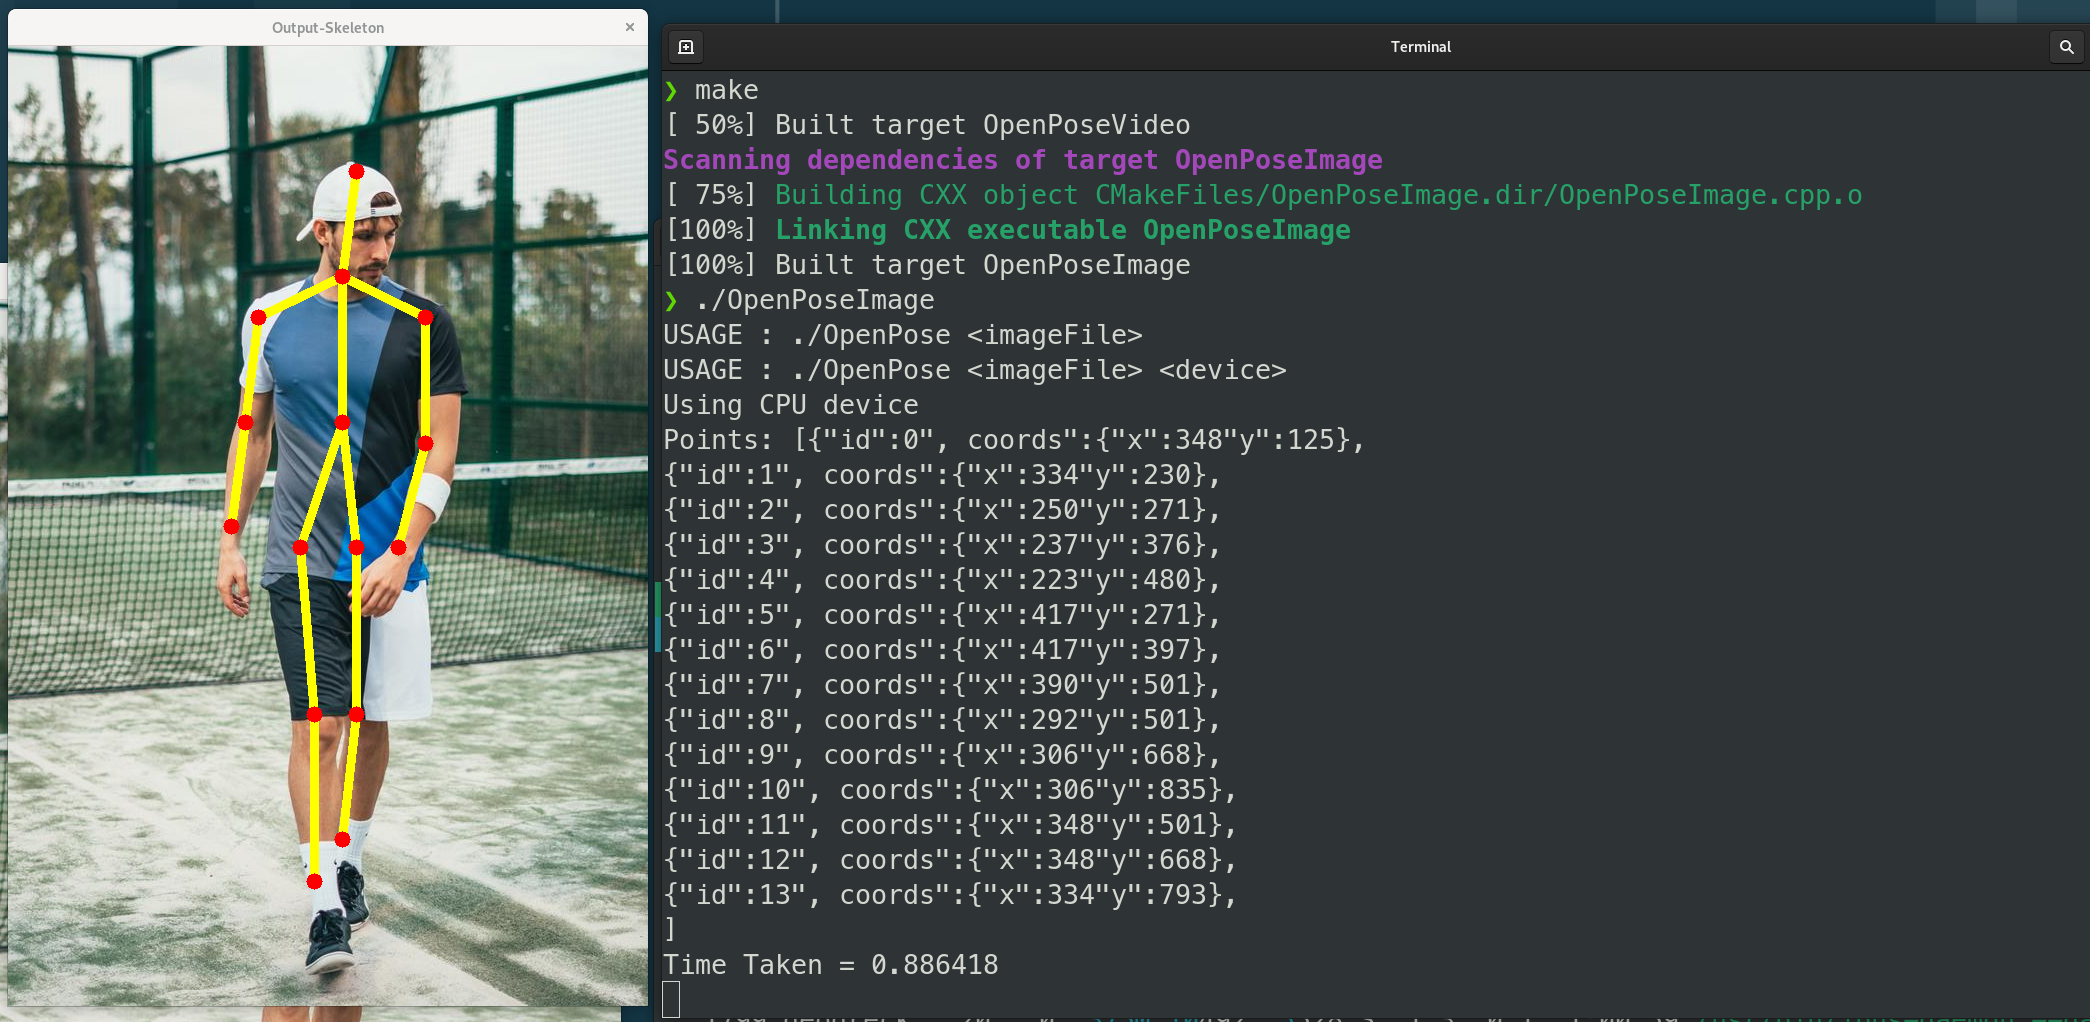
\includegraphics{pics/hw2_cppBody_out.png}
\caption{Реализация на C++}
\end{figure}

\hypertarget{ux441ux440ux430ux432ux43dux435ux43dux438ux435-ux441ux43aux43eux440ux43eux441ux442ux438-ux440ux430ux431ux43eux442ux44b-ux430ux43bux433ux43eux440ux438ux442ux43cux430-ux440ux430ux441ux43fux43eux437ux43dux43eux432ux430ux43dux438ux44f-ux43aux438ux441ux442ux438-ux440ux443ux43aux438-ux43dux430-c-ux438-python}{%
\subsection{\texorpdfstring{Сравнение скорости работы алгоритма
распознования кисти руки на \textbf{\texttt{C++}} и
\textbf{\texttt{python}}}{Сравнение скорости работы алгоритма распознования кисти руки на C++ и python}}\label{ux441ux440ux430ux432ux43dux435ux43dux438ux435-ux441ux43aux43eux440ux43eux441ux442ux438-ux440ux430ux431ux43eux442ux44b-ux430ux43bux433ux43eux440ux438ux442ux43cux430-ux440ux430ux441ux43fux43eux437ux43dux43eux432ux430ux43dux438ux44f-ux43aux438ux441ux442ux438-ux440ux443ux43aux438-ux43dux430-c-ux438-python}}

Для измерения использовалась команда linux \textbf{\texttt{time}}. В
таблицу заносилось общее(total) время.

\begin{longtable}[]{@{}llll@{}}
\toprule
& picture1 & picture2 & picture3\tabularnewline
\midrule
\endhead
python & 0.750 & 1.401 & 1.633\tabularnewline
c++ & 0.713 & 1.411 & 1.643\tabularnewline
\bottomrule
\end{longtable}

Программы работают за примерно одинаковое время.

\vspace{10cm}

\hypertarget{ux441ux440ux430ux432ux43dux435ux43dux438ux435-ux441ux43aux43eux440ux43eux441ux442ux438-ux440ux430ux431ux43eux442ux44b-ux440ux430ux437ux43dux44bux445-ux430ux43bux433ux43eux440ux438ux442ux43cux43eux432-ux440ux430ux441ux43fux43eux437ux43dux430ux432ux430ux43dux438ux44f-ux43aux438ux441ux442ux438-ux440ux443ux43aux438-ux43dux430-python}{%
\subsection{\texorpdfstring{Сравнение скорости работы разных алгоритмов
распознавания кисти руки на
\textbf{\texttt{python}}}{Сравнение скорости работы разных алгоритмов распознавания кисти руки на python}}\label{ux441ux440ux430ux432ux43dux435ux43dux438ux435-ux441ux43aux43eux440ux43eux441ux442ux438-ux440ux430ux431ux43eux442ux44b-ux440ux430ux437ux43dux44bux445-ux430ux43bux433ux43eux440ux438ux442ux43cux43eux432-ux440ux430ux441ux43fux43eux437ux43dux430ux432ux430ux43dux438ux44f-ux43aux438ux441ux442ux438-ux440ux443ux43aux438-ux43dux430-python}}

Методика тестирования та же.

\begin{longtable}[]{@{}llll@{}}
\toprule
& picture1 & picture2 & picture3\tabularnewline
\midrule
\endhead
1 module & 0.785 & 0.769 & 0.734\tabularnewline
2 module & 0.846 & 1.463 & 1.652\tabularnewline
\bottomrule
\end{longtable}

Первая программа на более сложных изображениях работает ощутимо быстрее.

\hypertarget{ux438ux437ux43eux431ux440ux430ux436ux435ux43dux438ux44f-ux43aux43eux442ux43eux440ux44bux435-ux438ux441ux43fux43eux43bux44cux437ux43eux432ux430ux43bux438ux441ux44c-ux432-ux445ux43eux434ux435-ux440ux430ux431ux43eux442ux44b}{%
\subsection{Изображения, которые использовались в ходе
работы:}\label{ux438ux437ux43eux431ux440ux430ux436ux435ux43dux438ux44f-ux43aux43eux442ux43eux440ux44bux435-ux438ux441ux43fux43eux43bux44cux437ux43eux432ux430ux43bux438ux441ux44c-ux432-ux445ux43eux434ux435-ux440ux430ux431ux43eux442ux44b}}

\begin{figure}
\centering
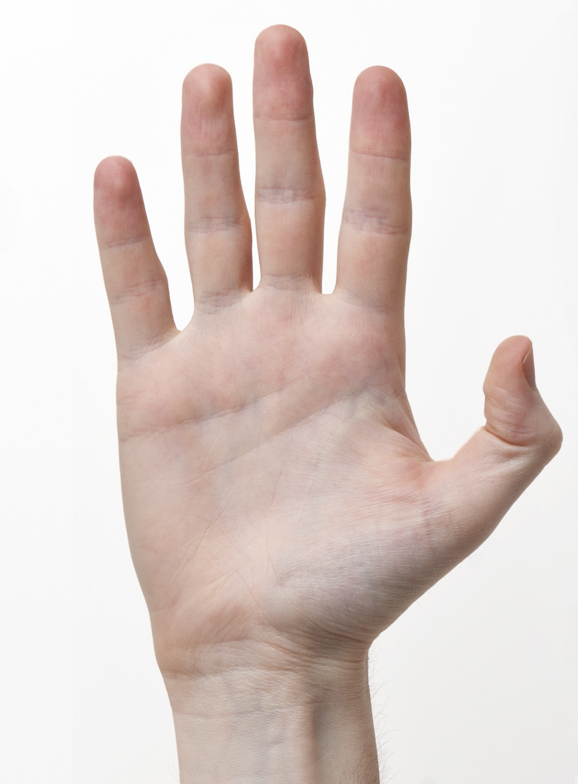
\includegraphics{../hw2/HandPose/right-frontal.jpg}
\caption{picture 1}
\end{figure}

\begin{figure}
\centering
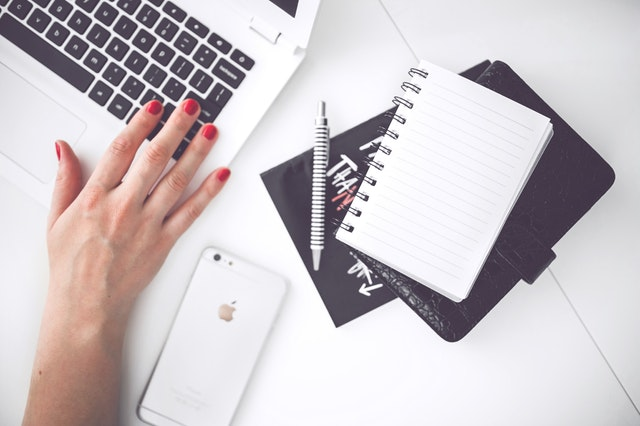
\includegraphics{../hw2/HandPose/hand.jpg}
\caption{picture 2}
\end{figure}

\begin{figure}
\centering
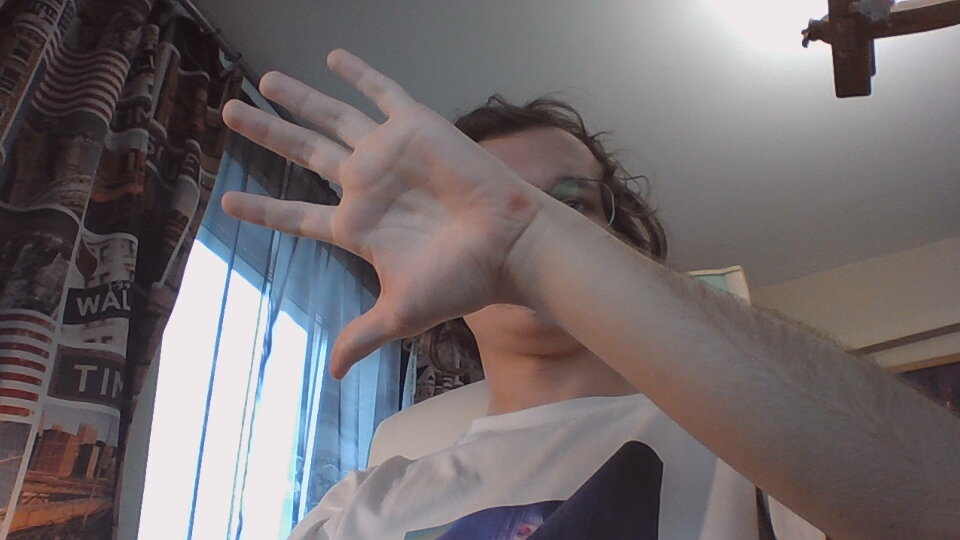
\includegraphics{../hw2/HandPose/myhand.jpg}
\caption{picture 3}
\end{figure}

\hypertarget{ux432ux44bux432ux43eux434ux44b}{%
\section{Выводы}\label{ux432ux44bux432ux43eux434ux44b}}

Существенной разницы в скорости работы распознования с помощью нейронной
сети на \textbf{\texttt{C++}} и \textbf{\texttt{python}} нет.

Однако нейронная сеть работает гораздо медленее алгоритма распознования
изображения из 1 модуля.

Но у нее есть свои преимущества, например, нейронная сеть дает более
точный результат, который можно ещё улучшить путем ее дальнейшего
обучения.

Алгоритм первого модуля в свою очередь позволяет обрабатывать
изображение в реальном времени, благодаря своей скорости.

\end{document}
